\documentclass[conference]{IEEEtran}
\IEEEoverridecommandlockouts
% The preceding line is only needed to identify funding in the first footnote. If that is unneeded, please comment it out.
\usepackage{cite}
\usepackage{amsmath,amssymb,amsfonts}
\usepackage{algorithmic}
\usepackage{graphicx}
\usepackage{textcomp}
\usepackage{xcolor}
\usepackage{underscore}
\usepackage[linesnumbered,ruled,vlined]{algorithm2e}
\usepackage{caption}
\usepackage{tabularx}
\usepackage{algorithmic}
\usepackage{subfigure}
\usepackage{float}
\usepackage{url}
\usepackage{pifont}
\def\BibTeX{{\rm B\kern-.05em{\sc i\kern-.025em b}\kern-.08em
    T\kern-.1667em\lower.7ex\hbox{E}\kern-.125emX}}
\SetNlSty{}{}{\scriptsize:}
\begin{document}

\title{Maat: A Fair and Scalable Layer-4 Load Balancer With Per-Connection-Consistency\\
	Paper id 216
}


\maketitle

\begin{abstract}
Layer-4 load balancers play a pivotal role in data centers by efficiently distributing incoming traffic across thousands of servers. These load balancers need to meet two key requirements: load balancing fairness, which ensures a uniform distribution of incoming traffic across servers, and per-connection-consistency (PCC), which guarantees that all packets belonging to the same connection are forwarded to the same server. Existing load balancers face a dilemma: they either sacrifice fairness to significantly reduce PCC violations, failing to meet both requirements, or they adopt complex scheduling mechanisms, which increase deployment and operational costs. In this paper, we introduce Maat, a load balancer designed to achieve fair load distribution and PCC while seamlessly integrating into existing data center infrastructures. Maat introduces a novel scheduling method called the power of one random choice. This method improves the utilization of all available servers, greatly enhancing load distribution fairness while reducing PCC violations. Furthermore, Maat can fully guarantee PCC by utilizing counting Bloom filters with negligible memory overhead. We implement Maat on a Tofino switch, and our experimental results show that the packet processing overhead of Maat is acceptable. Compared to other Layer-4 load balancers, Maat improves load balancing fairness by up to 74.42\% and reduces flow completion time by 10.58\%, while fully guaranteeing PCC at the cost of minimal memory consumption.
\end{abstract}

\begin{IEEEkeywords}
layer-4 load balancer, fairness, per-connection-consistency, programmable switch
\end{IEEEkeywords}

\section{Introduction}
In recent years, there has been a noticeable trend for businesses and enterprises to migrate services such as online searches and online games to cloud environments \cite{yao2022hlb}. This shift has driven the deployment of massive data centers to meet the growing demand for cloud services. However, simply providing the abundant link and server resources \cite{greenberg2009vl2} is no longer sufficient to meet the rapidly growing user needs. It can even be counterproductive if incoming traffic is not allocated resources adequately for processing. Recognizing the need for more reliable and scalable services, operators have begun to deploy load balancing mechanisms within data centers. For instance, a Layer-4 load balancer (L4 LB) ensures that incoming traffic is distributed fairly across all reachable backend servers (DIPs). The goal of L4 LB is to maximize resource utilization to meet the growing needs of the business.

Approximately half of data center traffic requires L4 LB for processing \cite{patel2013ananta}.  Inefficient handling of this traffic by L4 LB can have severe consequences for the data center. Potential outcomes include some servers being underutilized, resulting in resource wastage, while others become overloaded, leading to downtime or even service interruptions. These issues can further cause a sharp decline in user experience \cite{miao2017silkroad}. Therefore, in Layer-4 load balancing, fairness should be treated as a first-class citizen.

Effective management of incoming traffic by L4 LB encounters two significant challenges. The first challenge arises from skewed traffic distribution. Applications commonly utilize short connections for synchronization and long connections for massive data transfer, resulting in a long-tail distribution where a few flows carry the majority of the traffic \cite{zeng2022tiara}. Improper handling of L4 LB in such scenarios can easily lead to uneven load distribution among servers \cite{aghdai2020spotlight}. The second challenge stems from the limitations imposed by L4 LB when dealing with stateful protocols, such as TCP and QUIC \cite{langley2017quic}. These protocols are usually connection-oriented to improve communication reliability. Consequently, all packets of a flow must be processed by the same server to maintain \emph{per-connection-consistency} (PCC) \cite{miao2017silkroad}. PCC violations can cause connection interruptions and increase the end-to-end delay during connection re-establishment, significantly impacting service quality. To address these challenges, previous works have focused on maintaining PCC \cite{eisenbud2016maglev, olteanu2018stateless, gandhi2014duet, araujo2018balancing}. However, some studies have revealed that these schemes often reduce PCC violations at the expense of load distribution fairness \cite{barbette2021cheetah}, contradicting the fundamental purpose of L4 LB.


In general, LB primarily enhances fairness in two main ways. The first method involves adjusting the scheduling granularity, commonly utilized in L3 LB \cite{aghdai2020spotlight}. Operators often use flowlet-level \cite{alizadeh2014conga, katta2016hula, liu2023burstbalancer} or packet-level \cite{perry2014fastpass} granularity to improve fairness. However, in L4 LB, since all packets of the same connection must be forwarded to the same server to maintain PCC, the granularity is limited to the flow-level. The second approach is to choose different scheduling methods, such as hashing \cite{miao2017silkroad, gandhi2014duet}, round-robin \cite{katta2016clove, he2015presto}, the least congestion \cite{alizadeh2014conga, curtis2011mahout}, and so on. However, because of PCC limitations, L4 LB must maintain the mapping between flows and servers in dynamic network environments \cite{araujo2018balancing}.
Consequently, existing solutions typically rely on hashing, which is usually difficult to achieve good fairness, or requires modifications to the TCP/IP protocol stack in terminal devices to select other advanced scheduling methods. Although the latter can bring better fairness, it often has poor scalability and is difficult to deploy directly in existing data centers.

Based on the above discussion, we believe that L4 LB should meet the following requirements: 1) \textbf{Fairness}: fully utilize the available resources of all servers; 2) \textbf{PCC}: packets belonging to the same connection are forwarded to the same server; 3) \textbf{Scalability}: no changes to the end host or protocol stack during deployment. To achieve these goals, this paper proposes Maat, an L4 LB implemented on a programmable switch. Maat proposes a novel scheduling method termed the power of one random choice. Specifically, to enhance fairness, Maat processes each flow by selecting one of two servers for forwarding, with one server selected through hashing to maintain PCC. To further improve fairness, Maat also employs a finer-grained approach to capture and analyze the status information of incoming traffic directly, making the selection more accurate.

Using the power of one random choice while always maintaining PCC on Maat is challenging. To address PCC violations caused by DIP pool updates (i.e., removal or additional of servers), we adopt Othello hashing, a minimum perfect hash \cite{majewski1996family}, as our hashing function for server selection. It is typically used for load balancing with low memory overhead and no false hits \cite{yu2018memory}. Additionally, the power of one random choice also cause PCC violations due to random selection. We transform this problem into a membership set problem and introduce a counting Bloom filter\cite{bonomi2006improved} to ensure PCC. By cleverly combining Othello hashing with counting Bloom filters, Maat can fully guarantee PCC with negligible memory even under heavy load.


To summarize, the key contributions of Maat are as follows:
\begin{itemize}
	\item We show that existing scheduling methods often face a dilemma: they either sacrifice fairness to guarantee PCC or cannot be directly deployed in contemporary data centers. Consequently, we propose a novel scheduling method named power of one random choice, capable of satisfying the requirements of L4 LB for both fairness and PCC simultaneously.
	\item We design and implement Maat, an LB that meets the two key requirements of L4 LB. Maat is easy to implement in programmable hardware (e.g., Tofino switch \cite{barefoot2019}) and can be deployed without any changes to the end host or TCP/IP protocol stack.
	\item We evaluate Maat extensively in hardware testbed and conduct simulations in scenarios with realistic traffic patterns. Our experimental results show that Maat achieves significant improvement in fairness by 70-80\% compared to existing L4 LB under heavy load.
\end{itemize}

In \S II of this paper, we first summarize the advantages and disadvantages of previous L4 LB related work, then introduce the design motivation behind Maat, and finally, we present some background algorithms. Subsequently, we introduce the overall architecture and design details of Maat in \S III. Next, the implementation and experimental results of Maat are described in \S IV, and finally, we conclude Maat in \S V.

\begin{figure*}[htbp]
	\setlength{\abovecaptionskip}{0pt}
	\setlength{\belowcaptionskip}{-10pt}
	\begin{minipage}[t]{0.33\linewidth}
		\centering
		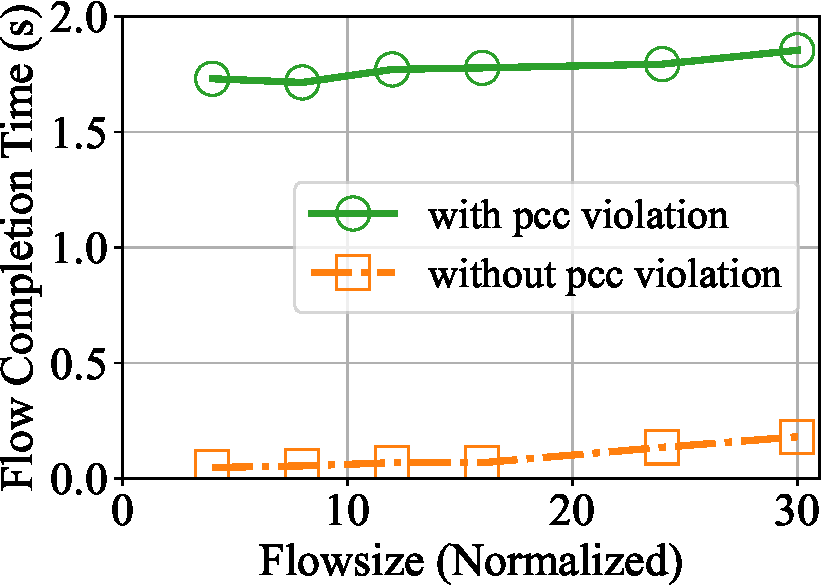
\includegraphics[width=1\textwidth]{experiment/0pccviolation.pdf}
		\caption{The impact of PCC violations.}
		\label{100}
	\end{minipage}%
	\centering
	\begin{minipage}[t]{0.33\linewidth}
		\centering
		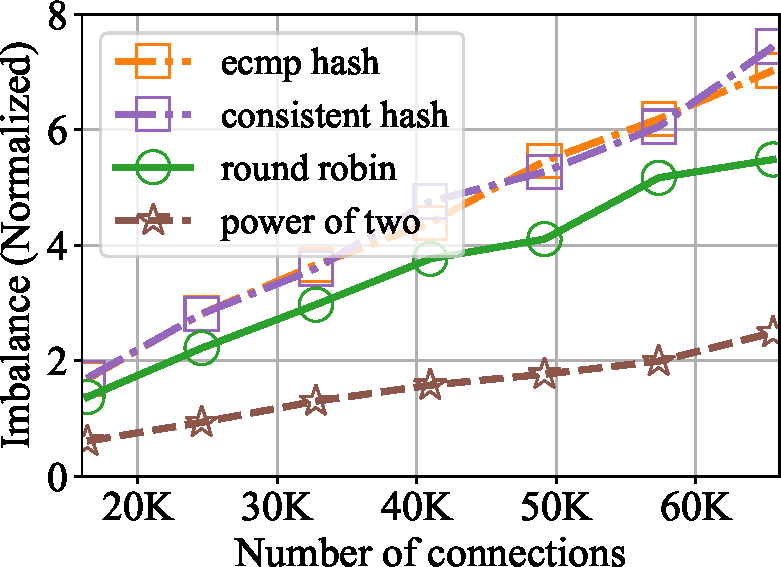
\includegraphics[width=0.977\textwidth]{experiment/1balancescheme.pdf}
		\caption{Load imbalance.}
		\label{2}
	\end{minipage}%
	\begin{minipage}[t]{0.33\linewidth}
		\centering
		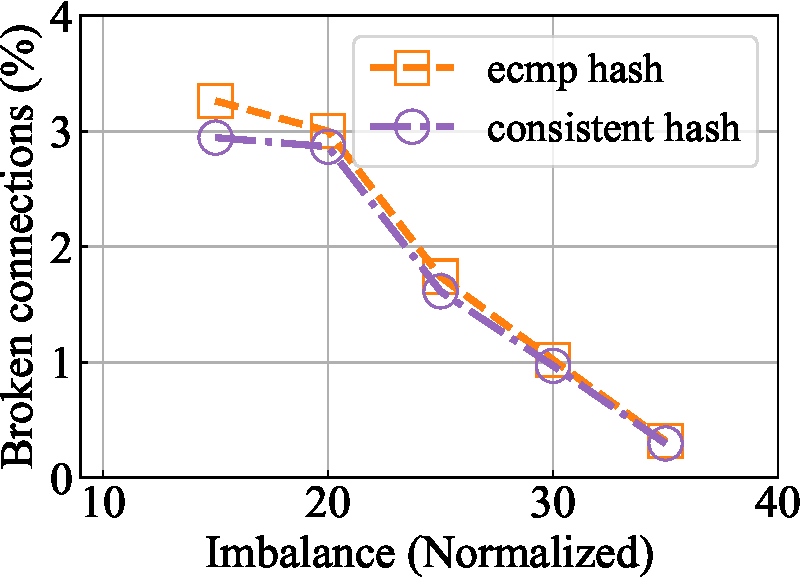
\includegraphics[width=0.988\textwidth]{experiment/2brokenimbalance.pdf}
		\caption{Relationship between broken connections and load imbalance.}
		\label{3}
	\end{minipage}
\end{figure*}

\section{BACKGROUND AND MOTIVATION}
Datacenter operators assign a virtual IP (VIP) address to each service they operate, and this virtual IP address is generally assigned to the L4 LB. Each VIP is associated with a set of servers (DIP pool) providing that service. The purpose of this paper is to design a simple and practical L4 LB scheme that evenly distributes incoming traffic across all available DIPs. In this section, we begin by presenting the advantages and disadvantages of both load-agnostic and load-aware L4 LB. Subsequently, we discuss the design motivation of Maat.
\subsection{Previous work}
\textbf{Load-agnostic L4 LB:}
Load-agnostic load balancers are characterized by relying on simple hash calculations\footnote{Hash algorithms refer to algorithms such as ECMP, consistent hashing, and minimum perfect hash.} to distribute incoming traffic among backend servers. Since these LBs do not consider the current load status of the servers, they often result in load imbalances. Research has shown that hash-based methods can suffer up to 30\% load imbalance \cite{eisenbud2016maglev}.

Solutions such as Ananta \cite{patel2013ananta}, Silkroad \cite{miao2017silkroad}, and Duet \cite{gandhi2014duet} all rely on ECMP hash to forward traffic, but these methods are prone to PCC violations when the DIP pool is updated. To solve this problem, solutions using consistent hashing such as Maglev \cite{eisenbud2016maglev}, Falid \cite{araujo2018balancing}, and Beamer \cite{olteanu2018stateless} are proposed. However, consistent hashing may introduce false hits during connection lookups due to the use of digests rather than complete state information. The occurrence of false hits may cause the L4 LB to forward packets to the wrong DIP, resulting in PCC violations. To address these problems, some works proposed applying Othello hashing to L4 LB \cite{yu2018memory}. For instance, Concury \cite{shi2020concury} and SDLB \cite{yu2017sdlb} are designed for cloud data centers and mobile edge computing, respectively. Due to the false-hit freedom characteristics of this hash algorithm, L4 LB can fully maintain PCC. Although load-agnostic LBs have made great progress in maintaining PCC. However, fairness as a first-class citizen in L4 LB has not received enough attention, and some schemes even ensure PCC at the expense of fairness.

\textbf{Load-aware L4 LB:}
Research in recent years has also realized that it is wrong for load-agnostic load balancers to sacrifice fairness to maintain PCC \cite{zhang2020fast, barbette2021cheetah, yao2022hlb}. As a result, some works have begun to strive to enhance fairness while maintaining PCC. The mainstream method is to adjust the weight of different servers through real-time network status (e.g., server status, traffic status), so that incoming traffic has a greater probability of selecting a more suitable server, thereby alleviating the load imbalance based on the hash scheme.

Server status-based methods collect information such as CPU and memory usage to guide forwarding strategies. However, they face three main challenges: 1) This type of solution is difficult to cope with the challenge of device heterogeneity and can easily cause L4 LB to make wrong forwarding decisions, thus damaging fairness \cite{zhang2020fast}. Here, device heterogeneity \cite{abdelmoniem2021towards} refers to the presence of multiple different devices within the same service. For server operators, a single service may be provided by multiple machines of various models \cite{sharma2011modeling}. Moreover, with the rise of cloud computing \cite{garg2014sla} and network function virtualization (NFV) \cite{lin2017enabling}, the device heterogeneity faced by contemporary cloud data centers may be more complex. 2) Server status-based solutions usually require additional high-performance equipment to implement complex interactions between LB and servers. For example, Spotlight \cite{aghdai2020spotlight} requires specifying an additional server (Intel i9 7900x with 64 GB RAM) as a dedicated controller for traffic management. 3) These methods also introduce security risks due to the frequent interactions required between the L4 LBs and servers to obtain accurate, real-time status updates. Third-party attackers can easily use sniffing attacks \cite{xiao2015detecting} to obtain server status information from frequent interactions, thereby conducting more targeted DDoS attacks \cite{garber2000denial}, causing some servers to go down or even the entire service to collapse. In summary, server state-based solutions not only face huge scalability challenges but also have difficulty handling potential security issues.

Another approach involves the load balancer directly collecting traffic status, which avoids complex interactions with servers, addresses potential security issues, and provides good scalability. However, there are also some problems with traffic state-based methods. For example, in LBAS \cite{zhang2020fast}, the scheduling policy relies on the number of active connections on the current server, ignoring the different effects of flow size on server load. Therefore, this approach runs the risk of forwarding incoming traffic to inappropriate servers. Although some methods \cite{guo2022libra} are aware of this problem, they still use a coarse-grained approach to collect traffic status information, which also leaves room for improper traffic allocation. To solve these problems, Maat introduces a more fine-grained traffic statistics method. With packet-level traffic statistics, incoming traffic can be assigned more accurate servers for better fairness.


\subsection{Motivation}
\textbf{PCC violations significantly increase the tail latency.} Maintaining PCC in L4 LB is crucial, as our experiments demonstrate that it has a significant impact on performance. We deployed HTTP service on three servers (1 client, 2 servers) and used a Tofino switch as the L4 LB. During this experiment, we generated workloads with increasing flow sizes and performed DIP pool updates. The experimental results in Fig. \ref{100} show that the FCTs with PCC violations are 10.28 times higher than those without PCC violations. This indicates that PCC violations severely affect the processing of incoming traffic, especially latency-sensitive traffic, potentially leading to unacceptable service level agreement (SLA) violations. From the experiment, it is clear that maintaining PCC is a prerequisite for L4 LB to improve fairness. However, we must ensure that load balance is not sacrificed to maintain PCC \cite{barbette2020high}.

\textbf{Hash-based L4 LB cannot spread incoming traffic evenly.} We compared hashing and other scheduling strategies for their ability to evenly distribute incoming traffic. The workload is generated based on the traffic distribution of Web search \cite{alizadeh2010data}. The experimental results are shown in Fig. \ref{2}. Among the four commonly used strategies, the power of two choices exhibits significant advantages. Specifically, it performs 2.83 times better than hash/consistent hash and 2.21 times better than round-robin. However, the limitations of maintaining PCC make it challenging to directly implement methods like the power of two choices or round-robin in L4 LB environments. Cheetah proposed a method that requires modifying the TCP/IP protocol stack by encoding the selected server’s identifier into a cookie added to all the packet headers.

\textbf{Hash-based L4 LB cannot guarantee PCC and load balance at the same time.} We conducted a simple experiment to evaluate whether these hash-based L4 LB can simultaneously achieve the two goals of enhancing fairness and maintaining PCC. In this experiment, we used an imbalance threshold as input and removed/added the server from the DIP pool when the server load is above/below the threshold \cite{barbette2021cheetah}. We used the traffic distribution of Web search to generate 100K connections. Fig. \ref{3} illustrates the relationship between fairness and the ratio of broken connections. It is worth noting that even when the load imbalance (normalized) reaches 30, the ratio of broken connections remains around 1\%. This demonstrates that L4 LB faces a conflict between enhancing fairness and ensuring PCC. In existing hash-based schemes, a common approach is to sacrifice load balance \cite{eisenbud2016maglev, olteanu2018stateless}, which goes against the original purpose of load balancing.

In brief, these experiments demonstrate that existing schemes cannot meet the three requirements of L4 LB (fairness, PCC, scalability). This motivates us to propose a new L4 LB scheme.


\subsection{Background algorithms}
\textbf{Power of two choices} is a commonly used scheduling method in load balancing, and in Figure \ref{3} we can see that it can achieve better fairness. This algorithm, originally proposed by David G. Andersen and Michael Kaminsky \cite{mitzenmacher2001power}, significantly enhances load balancing performance in supermarket models with a single input queue and multiple output queues using a limited number of choices (e.g., d = 2) \cite{ghorbani2017drill}.

However, in L4 LB, two random choices make maintaining the mapping between connections and servers more complex \cite{zhang2021loom, barbette2020high}. Therefore, most existing solutions still use hash functions to select servers because the hash function helps mitigate PCC violations. Unlike the existing L4 LB, Maat uses a novel scheduling method inspired by the power of two choices termed the power of one random choice. The basic idea is to compare the load of one hash selected server and one randomly selected server and choose the one with less load to forward traffic. 


\textbf{Othello hashing} is a minimal perfect hashing algorithm \cite{yu2017othello, chazelle2004bloomier} that supports forwarding information base and load balancing in programmable networks, including two arrays as its data plane, and a construction program in its control plane, as the interaction protocols of the two planes \cite{shi2020concury}. Since the Othello hashing has the characteristics of fast query speed and no false hits \cite{yu2017sdlb}, which can help us maintain PCC. So we use it as the hash function of the power of one random choice. We use the example in Fig. \ref{4} to demonstrate the operation of constructing and querying Othello.

Construction in the Othello control plane.
In Fig. \ref{4}, two arrays \emph{A} and \emph{B} are constructed with \emph{$m_a$} and \emph{$m_b$} elements, respectively. Each array element is an \emph{l}-bit value. In this example, \emph{l} = 2 and assume \emph{$m_a$} = \emph{$m_b$} = 5 for better illustration. For each value \emph{i} in \emph{A} we place a vertex \emph{$a_i$}, and for each value \emph{j} in B we place a vertex \emph{$b_j$}. Two hash functions \emph{$h_a$} and \emph{$h_b$} are used to compute the hash values of all \emph{$f_i$}. Then, for each \emph{$f_i$}, we place an edge between the two vertices corresponding to its hash value. For example, \emph{$h_a(f_{\text{2}})$} = 3 and \emph{$h_b(f_{\text{2}})$} = 1, so place an edge connecting \emph{$a_3$} and \emph{$b_1$}. For a \emph{$f_i$} and its corresponding \emph{index}, Othello hashing requires that two connected elements $\emph{A}[\emph{$h_a(f_{\text{i}})$}] \oplus \emph{B}[\emph{$h_b(f_{\text{i}})$}] = \emph{index}$, where $\oplus$ is a bitwise exclusive OR (XOR). For \emph{$f_2$} in this example, \emph{$a_3$} $\oplus$ \emph{$b_1$} = $11_2$ = 3. Note that after placing the edges of all \emph{$f_i$}, the bipartite graph formed by all vertexes must be acyclic. If a cycle is found, the construction must find another pair of hash functions to reconstruct the bipartite graph. It has been proved that the expected time cost of constructing a bipartite graph with \emph{n} \emph{$f_i$} is O(\emph{n}) \cite{yu2018memory}.

Query in the Othello data plane.
The Othello query structure contains two arrays \emph{A} and \emph{B}, as shown in Fig. \ref{4}. To query the value of \emph{\emph{$f_{\text{1}}$}}, we need to compute \emph{$h_a$} and \emph{$h_b$}, which are mapped to \emph{$a_1$} of \emph{A} and \emph{$b_0$} of \emph{B}. We then compute the bit-wise XOR of two vertexes and get the \emph{index} is $00_2$. For each packet, only two memory accesses are required, that is, reading a value from arrays \emph{A} and \emph{B} respectively, which can achieve fast queries.

\begin{figure}[t]
	\setlength{\abovecaptionskip}{0pt}
	\setlength{\belowcaptionskip}{-10pt}
	\centering
	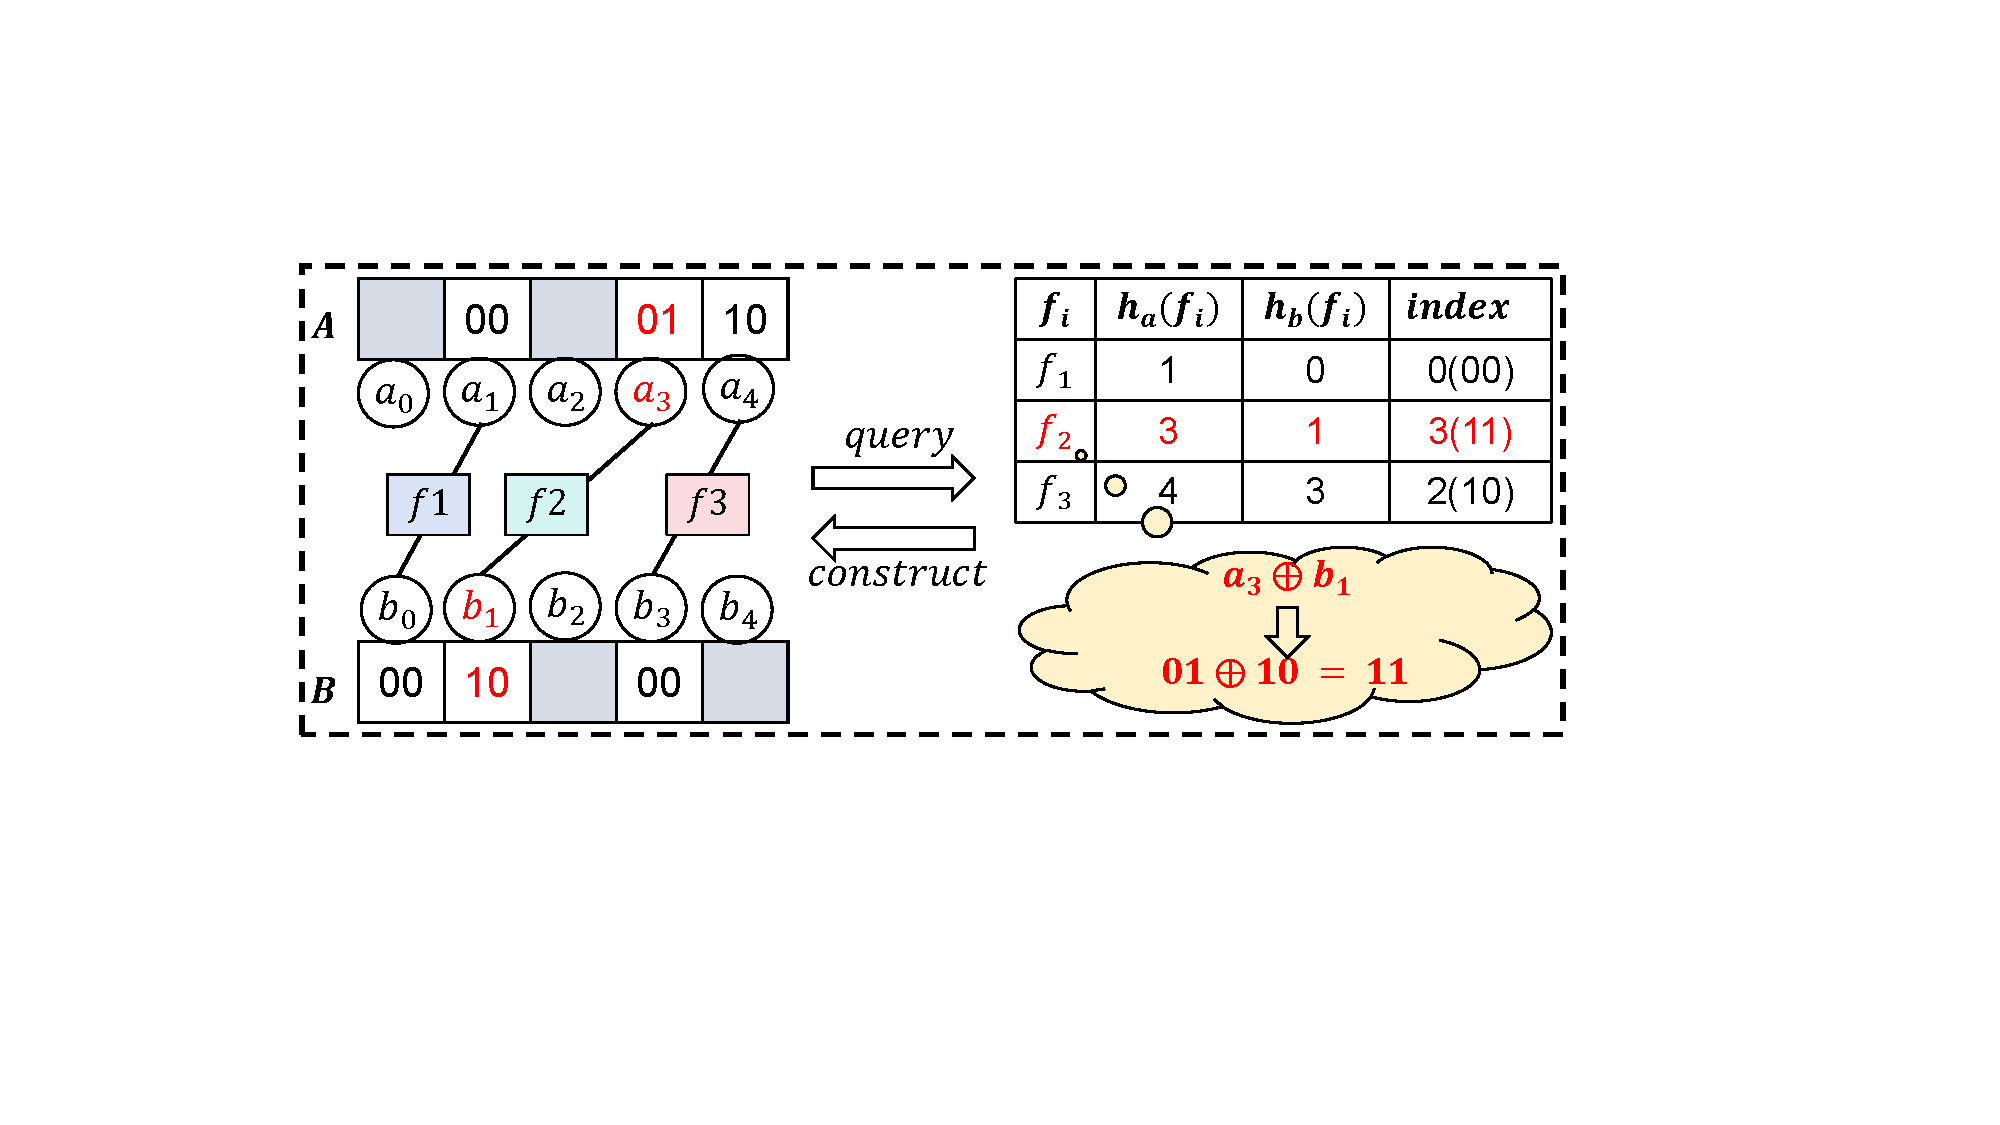
\includegraphics[width=1\linewidth]{figure/othello.pdf}
	\caption{The construction and query of Othello structure. \emph{$h_a$} and \emph{$h_b$} are the hash functions corresponding to the arrays \emph{A} and \emph{B} respectively.}
	\label{4}
\end{figure}

\section{DETAILS OF Maat}
In this section, we first outline the design rationale of Maat (\S III-A). Then the overall framework and workflow of Maat are described in detail (\S III-B \& \S III-C). Finally, the mechanism for Maat to fully maintain PCC is introduced (\S III-D). The main symbols used in Maat are shown in Table I.

\begin{table}[hbp]
	\centering
	\caption{Symbols frequently used in Maat.}
	\label{table1}
	\begin{tabular}{|m{1cm}<{\centering}|m{7cm}|}
		\hline
		Symbol & Description \\ \hline
		$\Delta$ & Flow size threshold used to identify load imbalance among servers \\ \hline
		\emph{$S_i$} & The \emph{$i^{th}$} server (DIP) \\ \hline
		\emph{$T[\emph{$S_i$}]$} & The total flow size of the \emph{$i^{th}$} server \\ \hline
		\emph{$B[\emph{$S_i$}]$} & The backup server of the \emph{$i^{th}$} server \\ \hline
		\emph{$F[\emph{$S_i$}]$} & Boolean value used to identify whether the \emph{$i^{th}$} server is acting as a backup server \\ \hline
	\end{tabular}
\end{table}

\subsection{Rationale of Maat} 
Maat is designed with two dimensions in mind: 1) Unlike existing L4 LBs that only use hash functions to select servers, Maat selects the less loaded server from two choices: one selected by hash and one selected randomly, which improves fairness. 2) Maat divides the incoming traffic into two categories, one is sent to hash-selected servers, and the other is sent to randomly selected servers. This approach helps resolve potential PCC violations with negligible memory overhead. By utilizing these two dimensions, Maat successfully meets both L4 LB requirements—maintaining PCC and improving fairness—without requiring modifications to the existing network infrastructure.


\begin{figure}[t]
	\setlength{\abovecaptionskip}{0pt}
	\setlength{\belowcaptionskip}{-10pt}
	\centering
	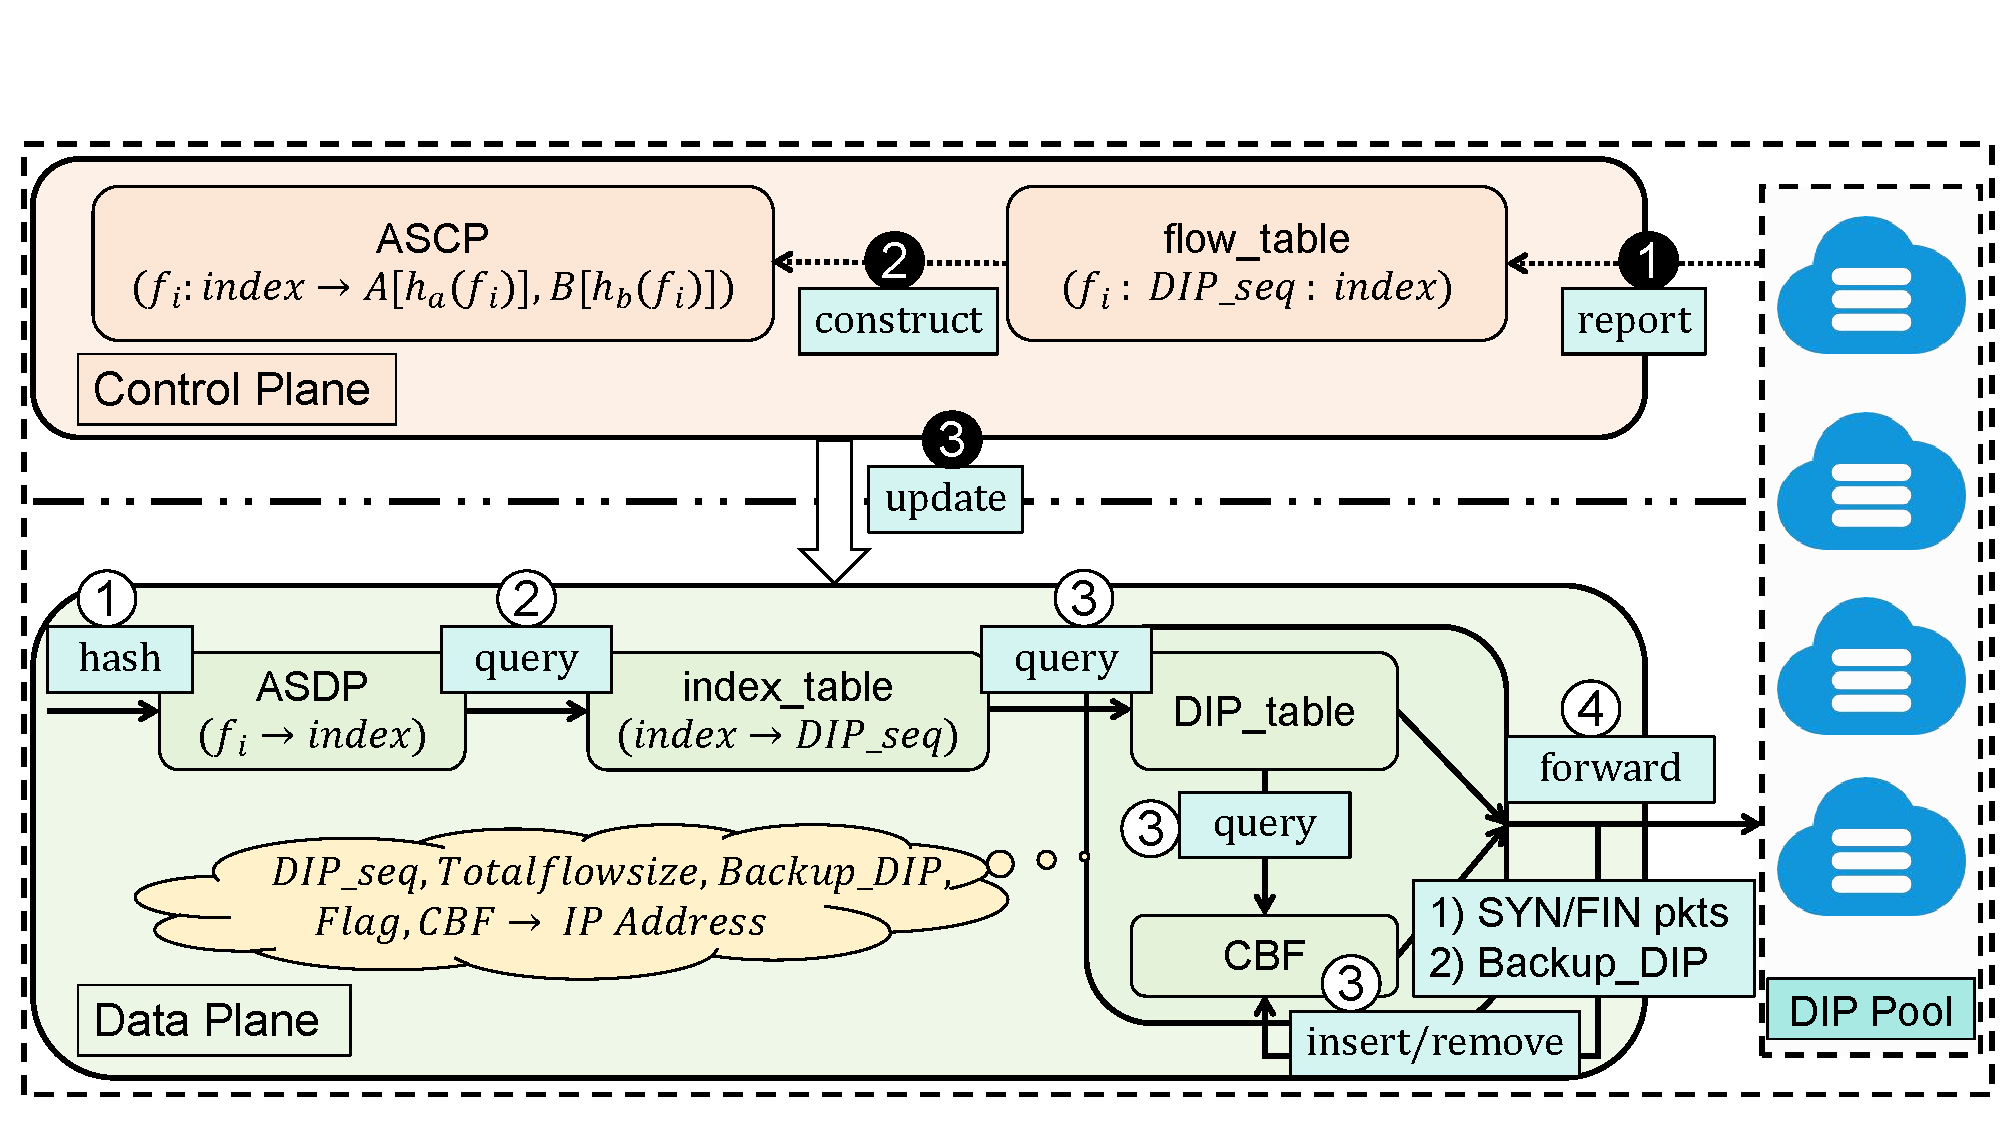
\includegraphics[width=1\linewidth]{figure/framework.pdf}
	\caption{Framework of Maat.}
	\label{5}
\end{figure}

\subsection{Frameworks of Maat}
Fig. \ref{5} shows the framework and workflow of Maat. In the data plane, we propose a scheduling method called the power of one random choice for enhancing fairness. Meanwhile, we also integrate Othello hashing and counting Bloom filters into Maat to mitigate potential PCC violations. In the control plane, our main concern is to update the data plane in real-time in response to changes in the DIP pool.

Maat is mainly composed of six major components:

(1) ASDP (Array Sets on Data Plane) is implemented by Othello hashing structure \cite{yu2018memory}, which consists of two arrays, \emph{A} and \emph{B}. Its main function is to query the corresponding \emph{index} for each flow. For example, with \emph{$f_{\text{3}}$} in Fig. \ref{4}, we first use \emph{$h_a$} and \emph{$h_b$} to calculate the hash values of \emph{$f_{\text{3}}$}, then use XOR to calculate \emph{A}[\emph{$h_a(f_{\text{3}})$}] (\emph{$a_4$}=$10_2$) and \emph{B}[\emph{$h_b(f_{\text{3}})$}] (\emph{$b_3$}=$00_2$). Finally, we can get that the \emph{index} corresponding to \emph{$f_{\text{3}}$} is 2.

(2) index\_table establishes a mapping relationship between \emph{index} and \emph{DIP_seq}. This is a many-to-one mapping \cite{olteanu2018stateless}, where multiple different \emph{index} values may map to the same \emph{DIP_seq}. \emph{DIP_seq} has a static mapping relationship with the IP address of the DIP. The \emph{index} is introduced to reduce memory consumption. Because the server's IP address is 32 bits, while the \emph{index} is usually much smaller, such as 8 bits \cite{shi2020concury}. Additionally, the number of \emph{index} mapped by each \emph{DIP_seq} can also be used to illustrate the weight (load status) of the server.

(3) DIP\_table is the core component of Maat and is responsible for forwarding packets to the appropriate server. It describes the status information of all servers (DIPs) running the same service. As shown in Fig. \ref{7}, it includes the following five fields: 1) \emph{DIP_seq}: A one-to-one mapping with the DIP's actual IP address. 2) \emph{IP Address}: The actual IP address of the DIP, is used to modify the destination IP address in the packet header. 3) \emph{Totalflowsize (T)}: Maat directly counts the number of packets of all flows processed on each server, rather than distinguishing which flows are large flows and which flows are small flows like the previous solution \cite{guo2022libra}. This method can more accurately reflect the impact of traffic on the server load (see Fig. \ref{9}). 4) \emph{Backup_DIP (B)}: This field is used to record the backup server of \emph{$S_i$}, The backup server \emph{$B[\emph{$S_i$}]$} is randomly selected to ensure load fairness among servers. As shown in Fig. \ref{7.2}, the backup server of \emph{$S_1$} is \emph{$S_2$}. 5) \emph{Flag (F)}: A boolean field, defaulting to false. When \emph{$S_1$} is selected as the backup for \emph{$S_2$}, the \emph{Flag} of \emph{$S_1$} is set to true to prevent other servers (e.g., \emph{$S_3$}) from selecting \emph{$S_1$} as their backup server. This field is introduced to achieve better load balancing between servers (see \S III-C1 for details).

(4) counting Bloom filter (CBF) is one of the variants of Bloom filter (BF) \cite{geravand2013bloom}. BF is a highly space-saving probabilistic data structure that enables efficient insertion and querying. CBF supports deletion operations based on BF, making CBF more suitable for dynamically changing data sets such as network traffic. CBF is primarily used to avoid potential PCC violations.

(5) flow\_table maintains the mapping relationship between \emph{$f_{\text{i}}$} and the server (DIP) on the control plane, recording the latest flows processed by the servers. It works by using a lightweight application-layer program to track the flow status of each server, which has been deployed to LB \cite{gandhi2014duet} in current data centers without changing the network stack. Whenever the flow status on the servers changes (e.g., flow arrival or termination), the servers report to LB, and then LB uses these reports to update flow\_table.

(6) ASCP (Array Sets on Control Plane) is also implemented by the Othello hashing structure but serves a different role than ASDP. Maat uses the latest mapping relationship in flow\_table to construct ASCP. Whenever the DIP pool updates, ASCP can quickly (microsecond level) update the data plane \cite{shi2020concury} to ensure that PCC violations not occur in Maat when the DIP pool changes, except in the case of server failure.

\subsection{Workflow of Maat}
(1) Data plane: The data plane of Maat is the key to achieving the two requirements (fairness \& PCC). For all incoming traffic, the LB selects an appropriate server among those running the corresponding service, rewrites the destination IP field in the packet header, and forwards it to the selected server. Maat's processing of packets is divided into two situations \cite{shi2020concury}: 1) Stateless packets. The flow to which the packet belongs has not selected any server. For example, for the first packet of each flow, LB needs to select a server for forwarding according to the pre-specified scheduling method; 2) Stateful packets. Unlike stateless packets, the flow to which the packet belongs has been processed. The LB needs to forward the packet to a specific server to ensure that all packets of the same connection are forwarded to the same server (PCC). Next, we describe in detail how the data plane handles these two types of packets.

1) Stateless packets: When Maat receives a stateless packet, such as the first packet (SYN=1) of a certain TCP flow (\emph{$f_i$}). We first query the \emph{index} corresponding to the flow in the ASDP (\ding{172}). Next, we find the \emph{DIP_seq} corresponding to the \emph{index} in the index\_table (\ding{173}), and finally, we find the hash-selected server in DIP\_table (assume {\emph{$S_1$}). We then process the stateless packets based on the power of one random choice (\ding{174}). We handle the following two situations according to Algorithm 1.
	
\begin{figure}[t]
	\setlength{\abovecaptionskip}{0pt}
	\setlength{\belowcaptionskip}{-10pt}
	\centering
	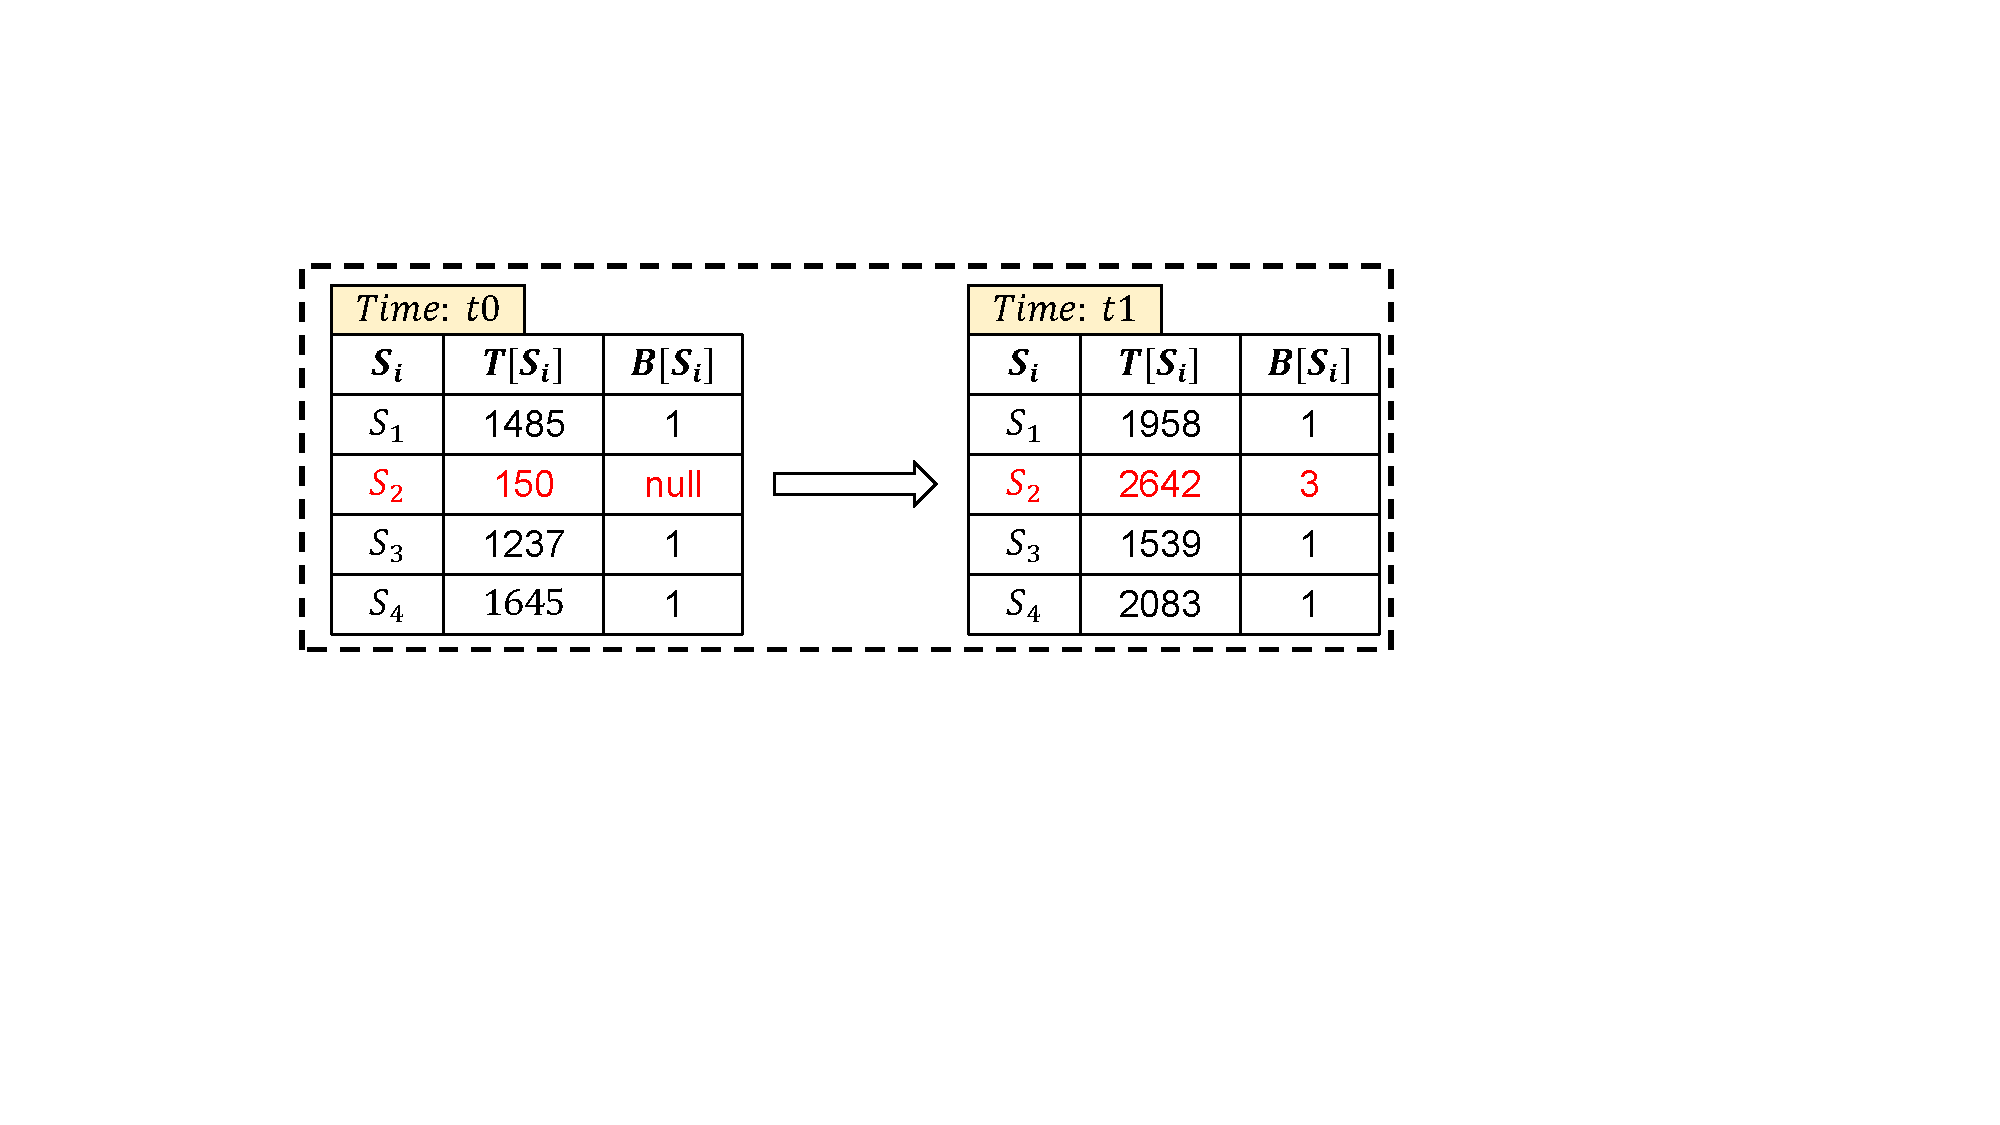
\includegraphics[width=1\linewidth]{figure/flag.pdf}
	\caption{Reason for introducing \emph{Flag} field in DIP_table ($\textbf{t1} > \textbf{t0}$, $\Delta = 1000 (packets)$).}
	\label{6}
\end{figure}

\textbf{Case 1.} \emph{B}[\emph{$S_1$}] is \emph{null}. In this case, \emph{$S_1$} may have a load imbalance with other servers, so we randomly select a server (assume \emph{$S_2$}). If $\emph{T}[\emph{$S_1$}] - \emph{T}[\emph{$S_2$}] \geq \Delta$ and $\emph{F}[\emph{$S_2$}] = \emph{false}$, where $\Delta$ is a predefined threshold indicating whether the flow should be forwarded to the backup server (Lines 1-8). The former condition shows that the load of \emph{$S_1$} is much greater than the load of \emph{$S_2$}, there is a load imbalance between \emph{$S_1$} and \emph{$S_2$}, and the latter indicates \emph{$S_2$} can serve as the backup server of \emph{$S_1$}. Thus, we set \emph{F}[\emph{$S_2$}] is \emph{true} and \emph{B}[\emph{$S_1$}] is \emph{$S_2$}, insert the flow into CBF (\ding{174}) to prevent PCC violation (see \S III-D for details), and finally forward the flow to \emph{$ S_2$} (\ding{175}). 

If either of the above two conditions is not met, i.e., $\emph{T}[\emph{$S_1$}] - \emph{T}[\emph{$S_2$}] \leq \Delta$ or $\emph{F}[\emph{$S_2$}] = \emph{true}$, it indicates that \emph{$S_1$} and \emph{$S_2$} may load balance or the load of \emph{$S_1$} is smaller than \emph{$S_2$}, or \emph{$S_2$} is already a backup server for other servers (Lines 9-11). In these cases, we should forward the packet to \emph{$S_1$} (\ding{175}) to achieve better fairness. We introduce the \emph{Flag} field in DIP_table to avoid scenarios like Fig. \ref{6}, where at \textbf{t0}, the load of \emph{$S_2$} is significantly lower than \emph{$S_1$}, \emph{$S_3$} and \emph{$S_4$}. Without the \emph{Flag} field, \emph{$S_2$} could be selected as a backup server by the other three servers. \emph{$S_2$} may handle too much load and become unbalanced with other servers at \textbf{t1}. This is caused by \emph{$S_2$} being selected as a backup server by multiple servers. In our tests, not introducing \emph{Flag} field lead to a 28.12\% decrease in fairness, and as the workload increases, this imbalance becomes more and more serious, especially in the case of long-tail distributions.

\textbf{Case 2.} \emph{B}[\emph{$S_1$}] is not \emph{null}. There may be a load imbalance between \emph{$S_1$} and \emph{B}[\emph{$S_1$}]. We compare the loads of \emph{$S_1$} and \emph{B}[\emph{$S_1$}]. If \emph{T}[\emph{$S_1$}] is much larger than \emph{T}[\emph{B}[\emph{$S_1$}]], and the difference exceeds $\Delta$, which means there is a serious load imbalance between \emph{$S_1$} and \emph{B}[\emph{$S_1$}] (Lines 12-16). Maat insert this flow into CBF (\ding{174}), forwarding the packet to \emph{B}[\emph{$S_1$}] (\ding{175}). On the contrary, it means that there is load balancing between \emph{$S_1$} and \emph{B}[\emph{$S_1$}], and the stateless packet is still forwarded to {\emph{$S_1$}} (Lines 17-19).

2) Stateful packets: When Maat receives a stateful packet (belonging to \emph{$f_i$}), our goal is no longer to select the appropriate server based on the scheduling method, but to ensure that the connection where the packet is located not be broken. Similarly, we find the correct \emph{index} and \emph{DIP_seq} in ASDP (\ding{172}) and index_table (\ding{173}) respectively. We can find the server selected by the hash function (assume \emph{$S_1$}). Next, we use the power of one random choice in the DIP_table  (\ding{174}) to handle the following two situations:

\textbf{Case 1.} \emph{B}[\emph{$S_1$}] is \emph{null} (Lines 20-22). In this case, \emph{$S_1$} has not selected any server as a backup server. We only need to forward the packet to \emph{$S_1$} (\ding{175}), which ensures that all packets belonging to the same connection are forwarded to the same server, that is, no PCC violation occurs.


\textbf{Case 2.} \emph{B}[\emph{$S_1$}] is not \emph{null} (Lines 23-29). To maintain PCC, we need to confirm that the currently processed flow is forwarded to \emph{$S_1$} or \emph{B}[\emph{$S_1$}]. Here, we use CBF (see \S III-D for details). If the flow record is found in CBF (\ding{174}), the flow is forwarded to \emph{B}[\emph{$S_1$}] (\ding{175}). If there is no related record, the flow is forwarded to \emph{$S_1$} (\ding{175}).

\begin{algorithm}[t]
	\caption{power of one random choice}
	\label{alg:example}
	\SetKwInOut{Input}{Input}
	\SetKwInOut{Output}{Output}
	
	\Input{A stateless/stateful packet of flow $f_i$, \\ 
		Hash selected server: \emph{$S_1$}, \\
		Threshold: $\Delta$}
	\Output{The server to handle the flow $f_i$}
	
	\tcp{A stateless packet of flow $f_i$}
	\If{ \emph{B}{$[\emph{$S_1$}]$} is null} {
		Random select server (\emph{$S_2$}); \\
		\If{ $\emph{T}[\emph{$S_1$}] - \emph{T}[\emph{$S_2$}] \geq \Delta$ \textbf{and} $\emph{F}[\emph{$S_2$}] = false$} {
			\emph{B}[\emph{$S_1$}] = \emph{$S_2$}; \\
			\emph{F}[\emph{$S_2$}] = \emph{true};  \\ \emph{T}[\emph{$S_2$}]++; \\
			\emph{CBF.insert($f_i$)}; \\
			\textbf{return} \emph{$S_2$};
		} \Else{
			\emph{T}[\emph{$S_1$}]++; \\
			\textbf{return} \emph{$S_1$};
		}
	} \Else{
		\If{$\emph{T}[\emph{$S_1$}] - \emph{T}[\emph{B$[\emph{$S_1$}]$}] \geq \Delta $} {
			\emph{T}[\emph{B$[\emph{$S_1$}]$}]++; \\
			\emph{CBF.insert($f_i$)}; \\
			\textbf{return} \emph{B}[\emph{$S_1$}]; \\
		} \Else{
			\emph{T}[\emph{$S_1$}]++; \\
			\textbf{return} \emph{$S_1$};
		}
	}
	
	\tcp{A stateful packet of flow $f_i$}
	\If{\textbf{B[\emph{$S_1$}]} is null} {
		\emph{$\emph{T}[\emph{$S_1$}]$}++; \\
		\textbf{return} \emph{$S_1$};
	} \Else{
		\If{${\emph{CBF.query($f_i$)}} = true$} {        \emph{T}[\emph{B$[\emph{$S_1$}]$}]++; \\
			\textbf{return} \emph{B}[\emph{$S_1$}];
		} \Else {
			\emph{T}[\emph{$S_1$}]++; \\
			\textbf{return} \emph{$S_1$};
		}
	}
\end{algorithm}

As shown in Fig. \ref{7.1}, the first packet of $f_1$ is hashed to select \emph{$S_2$}. Then, by using the power of one random choice, Maat randomly selects \emph{$S_1$}, and finally, forwards the first packet of $f_1$ to \emph{$S_2$} according to the judgment condition. Other situations can also be processed according to Algorithm 1, and the incoming packets are forwarded to the appropriate server to meet the requirements of L4 LB for fairness and PCC.

As seen from the workflow of the Maat data plane, the power of one random choice combines the advantages of the hash algorithm and the power of two choices cleverly. Initially, hash selection played a key role in significantly reducing PCC violations. At the same time, through one random choice, the utilization of all server resources is improved, thereby greatly enhancing load fairness among servers. Subsequent experiments demonstrate that this algorithm not only effectively preserves PCC but also enhances fairness.

(2) Control plane: The main task of the control plane is to promptly update the latest mapping relationship between flow and DIP to the data plane when the network changes. This function is similar to the control plane in most previous works \cite{miao2017silkroad, eisenbud2016maglev, zhang2021loom}.  The control plane interacts with the lightweight programs running on each server \cite{gandhi2014duet}. Whenever the control plane receives a report from the server, flow_table is updated (\ding{182}). Afterward, Maat(\ding{183}) constructs the latest ASCP through addition/deletion operations. The time complexity of related operations is \emph{$O(1)$} \cite{yu2018memory}. Whenever the DIP pool changes, the control plane can use ASCP to construct the latest ASDP for the data plane, clears the CBF, index\_table and DIP\_table is updated to forward traffic to the new DIP pool, where \emph{T},\emph{B} and \emph{F} of DIP_table are reset (\ding{184}).


\subsection{Keep PCC}
Related work \cite{shi2020concury} has mentioned that the Othello hashing structure can guarantee PCC regardless of network changes (e.g., DIP pool updates). However, when Maat applies this structure to hash selection in the power of one random choice mechanism, PCC violations may occur. In Fig. \ref{7.1}, the hash selection of \emph{$f_1$} is \emph{$S_2$}, but the random selection is \emph{$S_1$}. It is observed that there is a load balance between \emph{$S_2$} and \emph{$S_1$}, therefore, the packet is forwarded to \emph{$S_2$}. In Fig. \ref{7.2}, the hash selection of \emph{$f_2$} is \emph{$S_2$}, and the random selection is \emph{$S_3$}. However, there is a load imbalance between \emph{$S_2$} and \emph{$S_3$}, so Maat forwards \emph{$f_2$} to \emph{$S_3$} to alleviate the load imbalance. Although the hash selections for \emph{$f_1$} and \emph{$f_2$} are both \emph{$S_2$}, the final server selection is different: \emph{$f_1$} is forwarded to \emph {$ S_2$}, while \emph{$f_2$} is forwarded to \emph{$S_3$}. Each flow may have two choices: 1) a hash-selected server; or 2) a randomly selected server. If the selection of each flow cannot be distinguished, a PCC violation is likely to occur.

The basic approach involves utilizing an additional table to store the relationship between the connection and the backup server. However, to minimize memory usage, we can elegantly transform this key-value store challenge into a more simplified membership set problem \cite{gandhi2014duet}. For this problem, we adopt the counting Bloom filter (CBF) as a solution, CBF is a space-efficient random data structure that can efficiently determine whether an element belongs to a set. Specifically, when a flow is forwarded to the backup server, for SYN packets, we insert this flow into CBF, and for FIN packets, we remove this flow from CBF, and for other packets, we query CBF to confirm whether to forward them to the backup server. In Fig. \ref{7.3}, considering \emph{$f_1$} and \emph{$f_2$}, \emph{$f_2$} needs to be inserted into CBF. Then, for subsequent packets from \emph{$f_1$} and \emph{$f_2$}, a simple query in the CBF can determine whether to forward the packet to \emph{$S_2$} or \emph{$S_3$}, thus helping us avoid potential PCC violations. Furthermore, whenever the control plane updates the data plane, the data plane can maintain the latest mapping relationship, so we only need to clear CBF when updating the data plane. With the integration of CBF, Maat effectively addresses potential PCC violations with minimal memory overhead, even under heavy load.

    \begin{figure}[t]
	\setlength{\abovecaptionskip}{0pt}
	\setlength{\belowcaptionskip}{-10pt}
	\centering  %图片全局居中
	\subfigure[$f_1$ forward to \emph{$S_2$} (IP Address: 192.168.1.2).]{
		\label{7.1}
		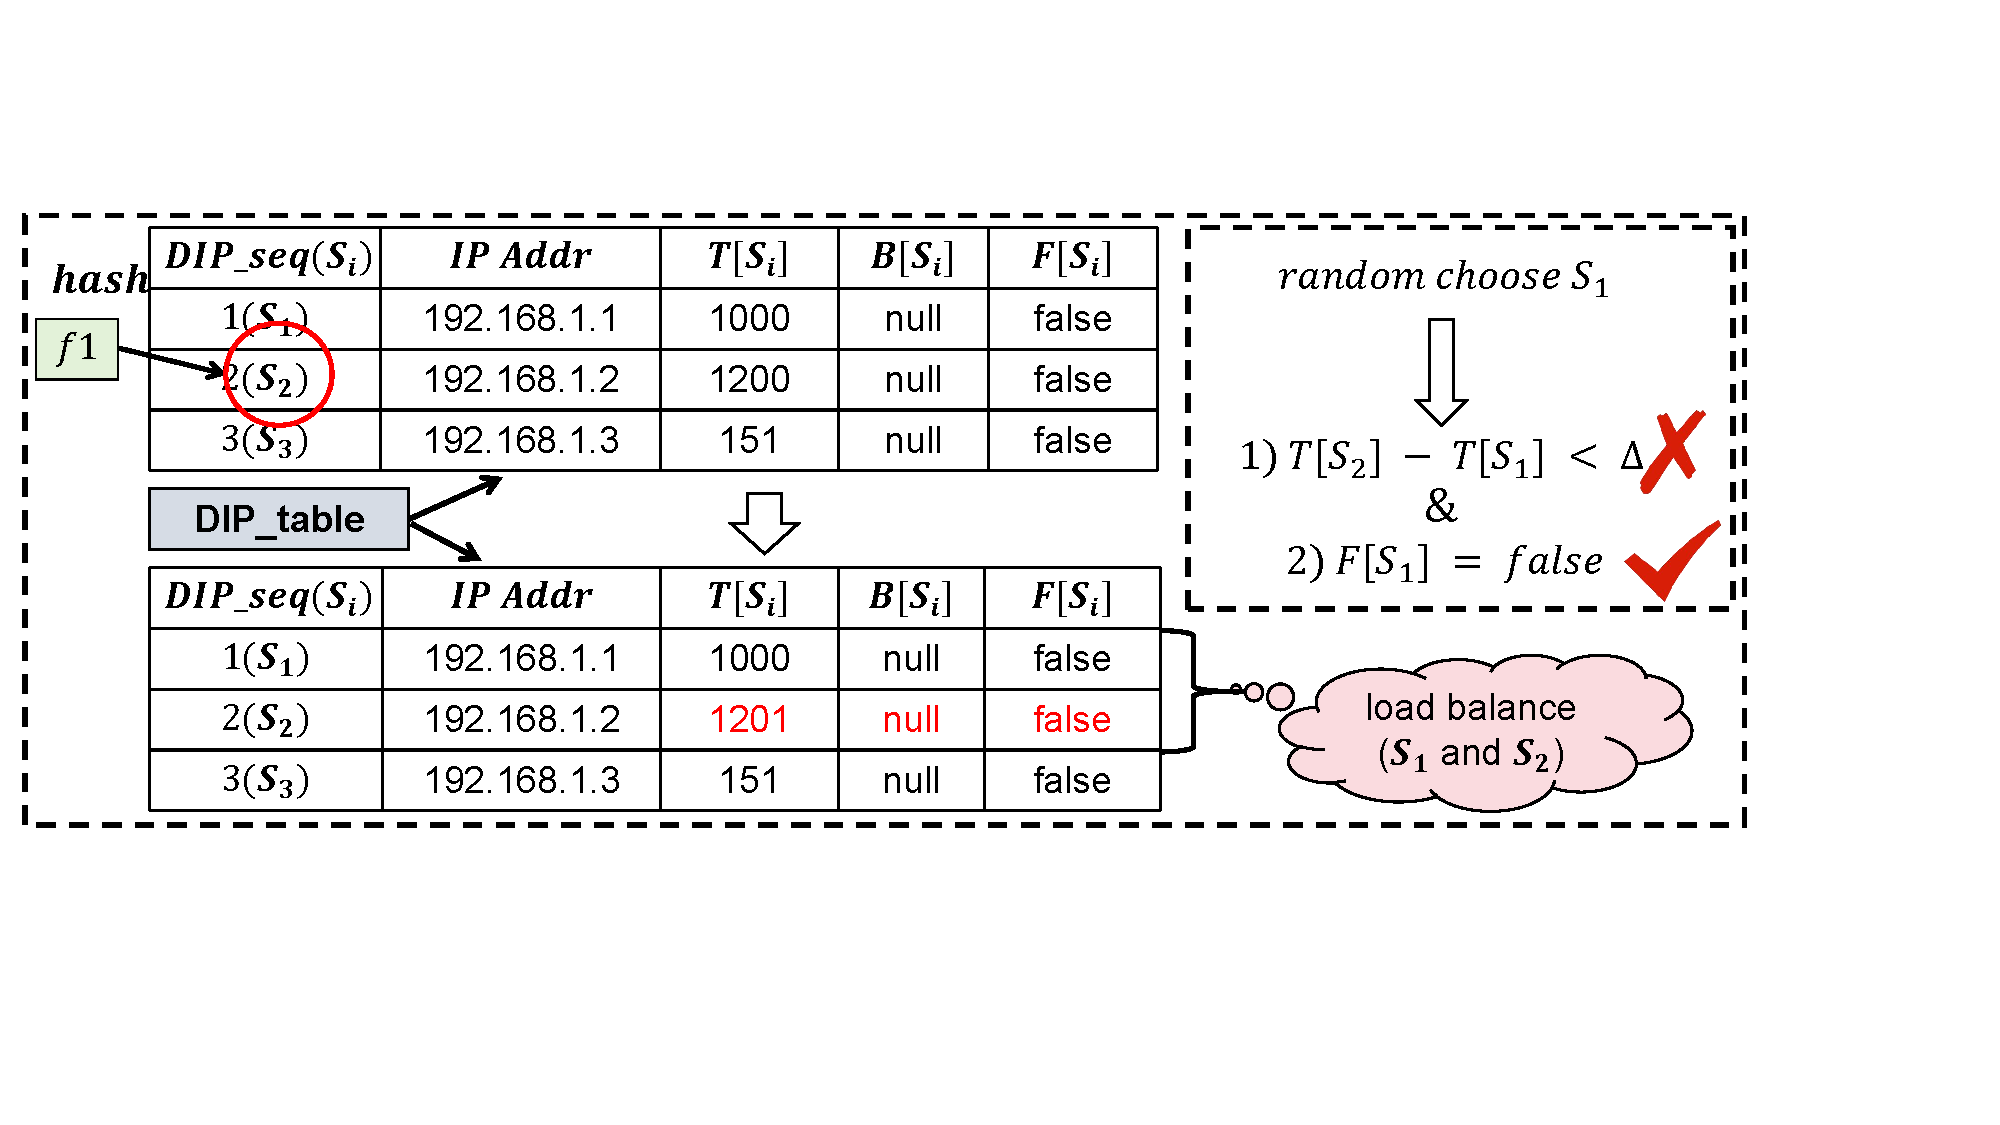
\includegraphics[width=1\linewidth]{figure/keeppcc1.pdf}}\\
	\subfigure[$f_2$ forward to \emph{$S_3$} (IP Address: 192.168.1.3).]{
		\label{7.2}
		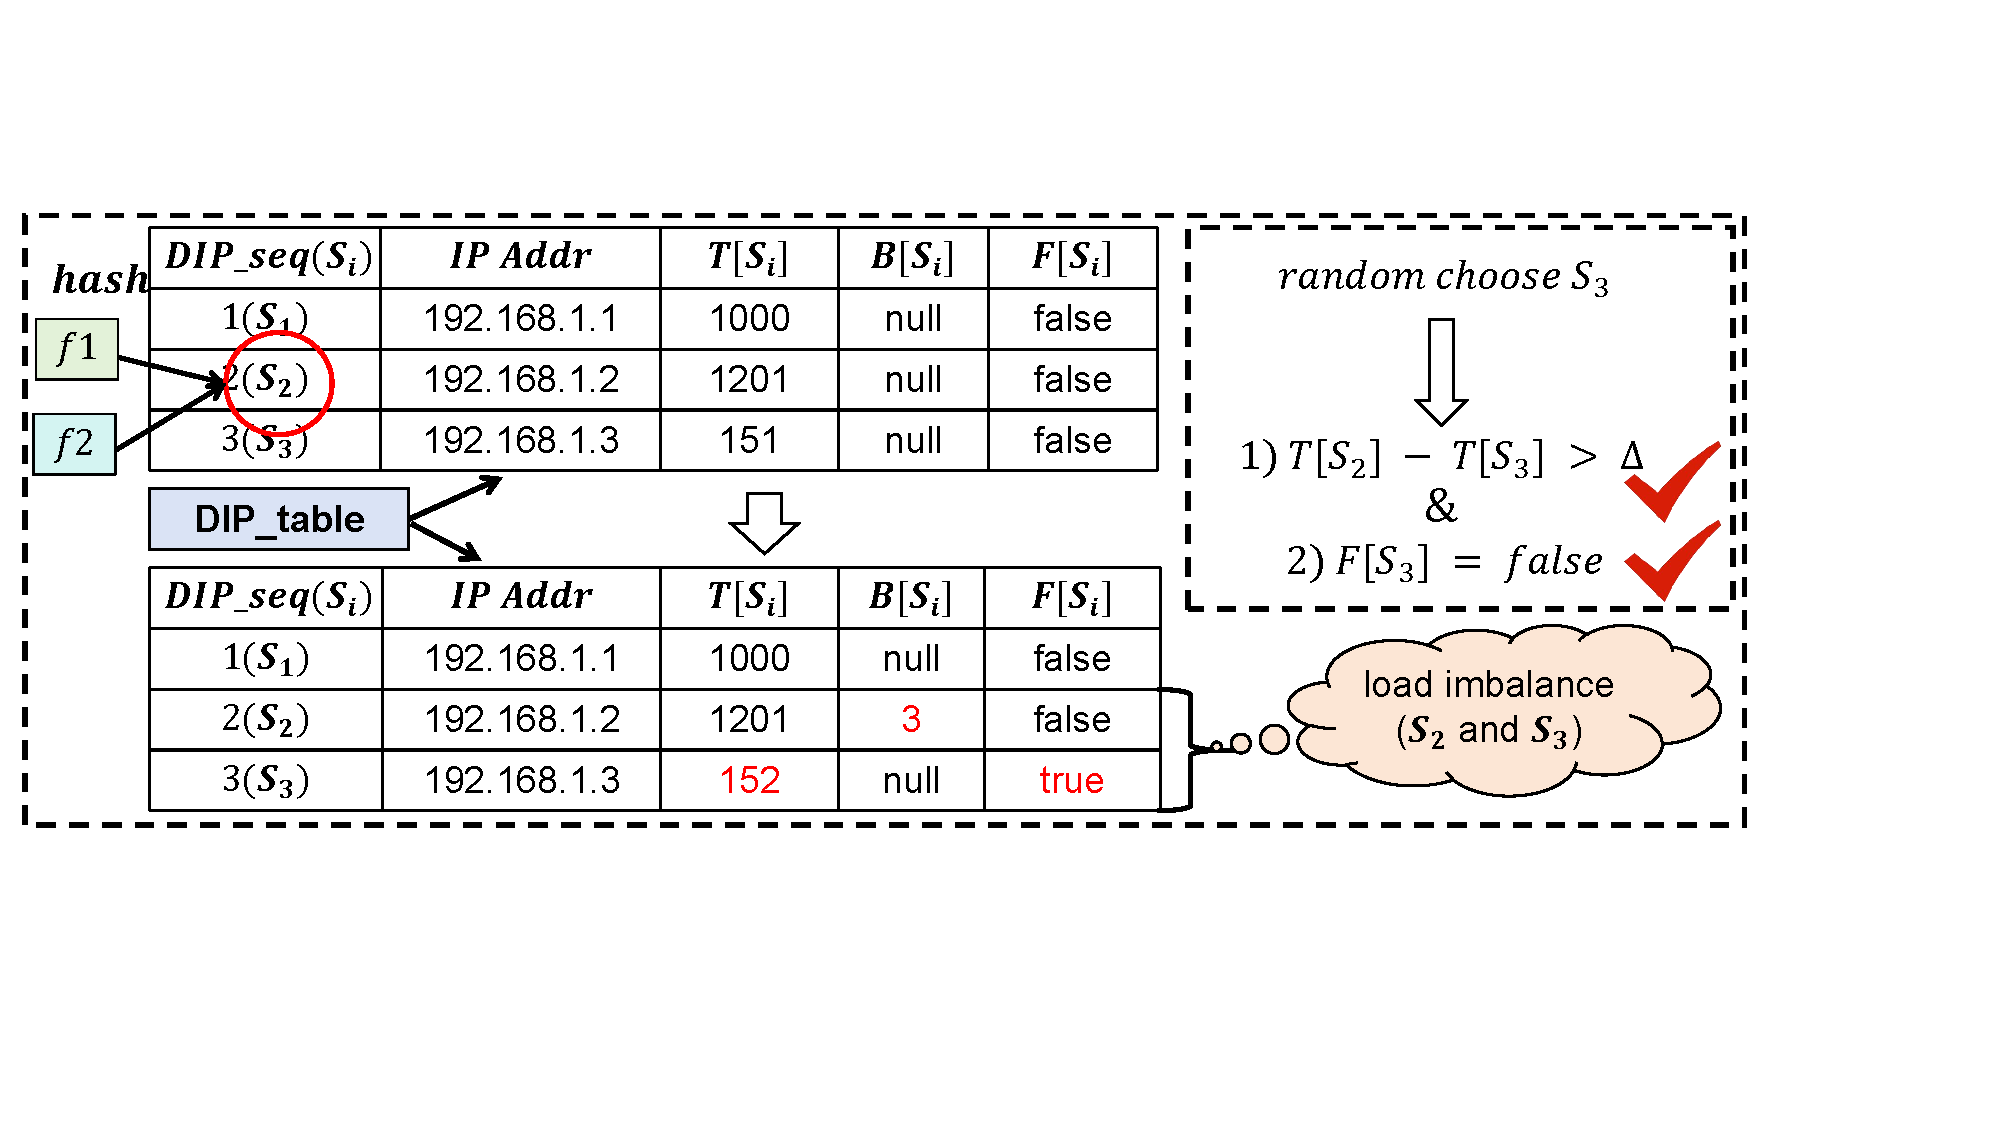
\includegraphics[width=1\linewidth]{figure/keeppcc2.pdf}}
	\subfigure[$f_2$ insert \textbf{CBF}.]{
		\label{7.3}
		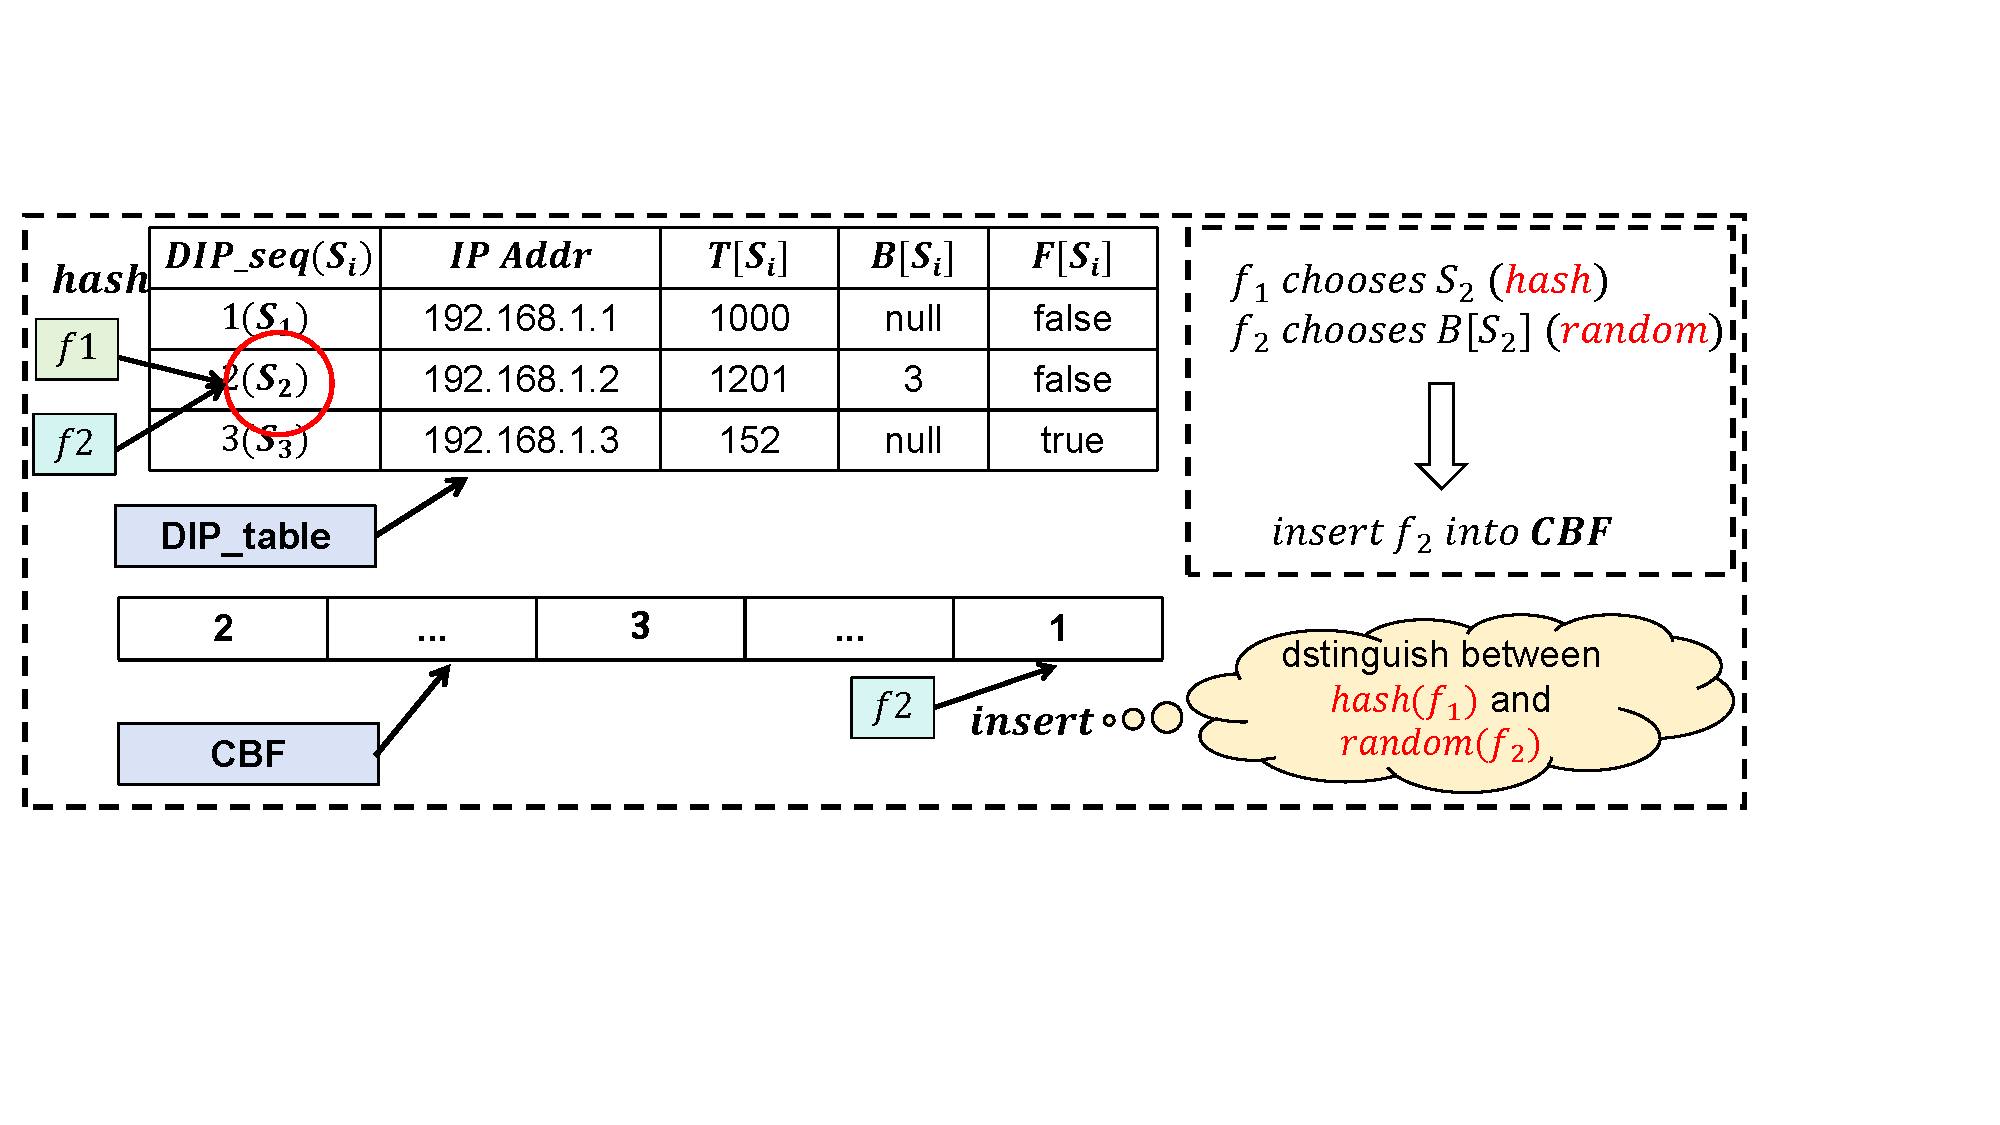
\includegraphics[width=1\linewidth]{figure/keeppcc3.pdf}}
	\caption{An example of keep PCC ($\Delta = 1000 (packets)$).}
	\label{7}
\end{figure}  

\begin{figure*}[ht]
	\setlength{\abovecaptionskip}{0pt}
	\setlength{\belowcaptionskip}{-10pt}
	\centering
	\subfigure[Web Search.]{
		\begin{minipage}[b]{0.46\textwidth}
			% height=1.7in, width=3in
			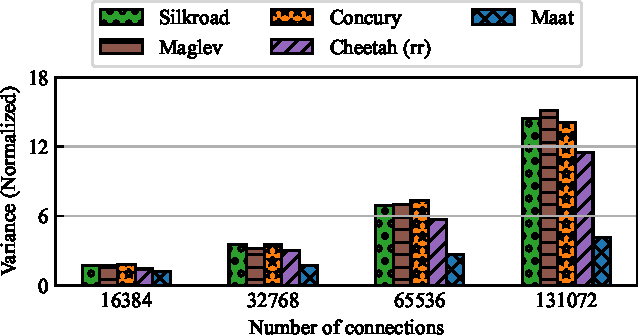
\includegraphics[width=1\linewidth]{experiment/3maatvarianceschemewb.pdf}
		\end{minipage}
		\label{8.1}
	}
	\subfigure[Data Mining.]{
		\begin{minipage}[b]{0.46\textwidth}
			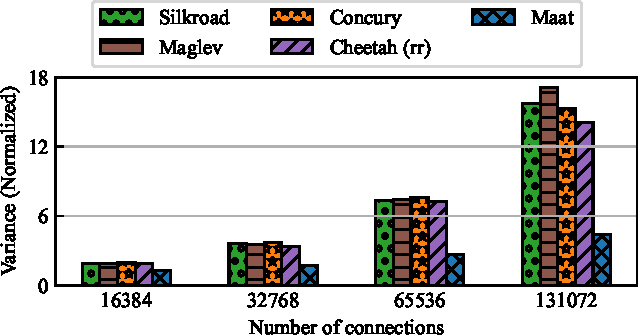
\includegraphics[width=1\linewidth]{experiment/3maatvarianceschemedm.pdf}
		\end{minipage}
		\label{8.2}
	}
	\vspace{0pt}
	\caption{Variance among servers’ load of various L4 LB schemes for increasing connections.}
	\label{8}
\end{figure*}

\begin{figure*}[ht]
	\setlength{\abovecaptionskip}{0pt}
	\setlength{\belowcaptionskip}{-10pt}
	\centering
	\subfigure[Web Search.]{
		\begin{minipage}[b]{0.46\textwidth}
			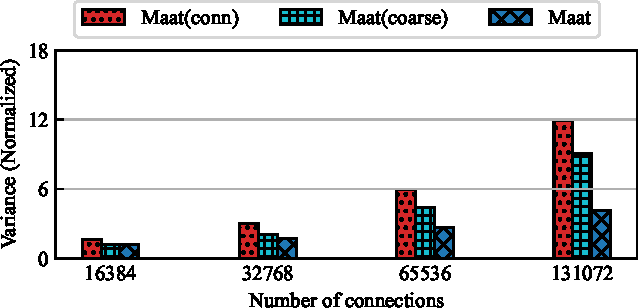
\includegraphics[width=1\linewidth]{experiment/4maatvariancegranwb.pdf}
		\end{minipage}
		\label{9.1}
	}
	\subfigure[Data Mining.]{
		\begin{minipage}[b]{0.46\textwidth}
			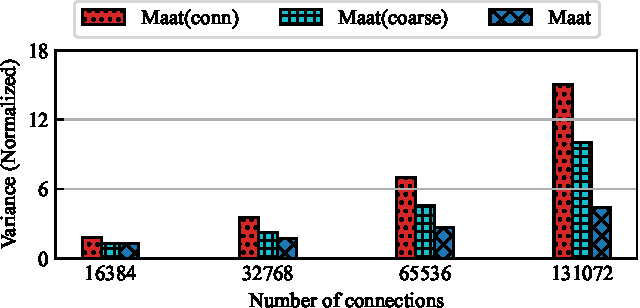
\includegraphics[width=1\linewidth]{experiment/4maatvariancegrandm.pdf}
		\end{minipage}
		\label{9.2}
	}
	\vspace{0pt}
	\caption{Variance among servers’ load of different collect traffic status methods for increasing connections.}
	\label{9}
\end{figure*}

\section{IMPLEMENTATION AND EVALUATION}
In this section, we evaluate the performance of Maat based on three types of evaluations: 1) algorithm micro-benchmark (\S IV-A); 2) Maat implemented based on DPDK (\S IV-B), and 3) Maat running on a Tofino switch (\S IV-C). Our experiments aim to answer the following questions.
\begin{itemize}
	\item[\textbf{1)}] \textbf{Can Maat achieve better fairness and guarantee PCC well?} (\S IV-A)
	\item[\textbf{2)}] \textbf{How does the performance of traffic processing in Maat?} (\S IV-B)
	\item[\textbf{3)}] \textbf{How does Maat perform on a Tofino switch?} (\S IV-C)
\end{itemize}

\textbf{Metric.} We evaluate the fairness across servers using both the variance of the server loads and the flow completion time (FCT). FCT refers to the time between the client initiating a connection and receiving the last ACK. Furthermore, we utilize memory overhead and processing throughput to evaluate the performance of Maat. We run at least 30 times for most experiments and take the average.

\textbf{Workload.} For algorithm evaluation (\S IV-A), we use two real workloads: 1) Web search workload \cite{alizadeh2010data} from a production cluster running web search service; 2) Data mining workload \cite{montazeri2018homa} containing many small flows. Both workloads are heavy-tailed: a small percentage of large flows contribute to most of the traffic. For testbed evaluation (\S IV-B and \S IV-C), We mainly use the following two tools to generate traffic to LB: 1) the  Pktgen-DPDK \cite{pktgenDPDK}; 2) the WRK \cite{glozer2020wrk}. We use a single server to run up to 32 NGINX web servers (one per hyper-thread), isolated using Linux network namespaces to allow packets to be accepted on the correct CPU core \cite{barbette2021cheetah}. We generate requests from clients using heavy-tailed distributions.

\textbf{Parameter selection.} We set the parameters of Maat intuitively: 1) We set the threshold $\Delta$ to 100K ($1K=1000$) packets. The reason for setting a larger threshold is that we found that using Maat with a larger $\Delta$ can not only use fewer resources to maintain PCC fully but also improve fairness. 2) For the setting of counting Bloom filter size, the main factor we consider is how many resources Maat requires to maintain PCC fully. We found that setting the size of CBF (2 bits per bucket) to 5.6KiB guarantees PCC even under heavy load. When deploying Maat in an actual operating environment, operators should fine-tune the settings of the above parameters according to changes in scenarios and requirements. In all cases, unless otherwise specified, we follow the settings of the above parameters.

\subsection{Evaluation of algorithm micro-benchmark}
 We comprehensively compare Maat with the following schemes: Silkroad \cite{miao2017silkroad}, Maglev \cite{eisenbud2016maglev}, Concury \cite{shi2020concury}, and Cheetah \cite{barbette2021cheetah}, where Cheetah chooses a round-robin mechanism for its scheduling method. These solutions are implemented based on the open-source code provided by \cite{cheetah} and \cite{concury2019}. The server used for the algorithm micro-benchmark experiment has an Intel(R) Xeon(R) Silver 4210R CPU, 2.40GHz, 128GB DDR4 memory, and 13.75MB L3 cache shared by 40 logical cores.
 
 \textbf{Fairness of different L4 LB schemes.} Fig. \ref{8} shows the fairness of different L4 LB schemes through the variance of the server loads. Silkroad \cite{miao2017silkroad} mentioned that the DIP pool in modern data centers is updated about 10 times per minute, which means that the data plane of LB is updated approximately every 6 seconds. Therefore, in the topology of 1 VIP and 32 DIP, we set the number of flows from 16K to 130K. This is according to the experimental settings of Cheetah \cite{barbette2021cheetah}. We found that under the same number of connections, Maat improves by 30.62\% to 74.42\% compared to other hash-based schemes. As the number of connections increases, the fairness issues of hash-based schemes become increasingly obvious, while Maat always maintains good fairness. Maat shows an improvement of 13.4\% to 63.26\% over Cheetah (rr). The above experimental results show that the fairness of Maat has been significantly improved compared with existing schemes, verifying that the scheduling method of power of one random choice can greatly improve fairness.
 
 \textbf{Fairness of different statistical methods.} Fig. \ref{9} illustrates the fairness of using different methods to count traffic states within the same LB scheme (Maat). This experiment compared three statistical methods: 1) Maat (conn): Counts only the number of connections, ignoring the difference in the impact of flow size on the server load. This can lead to load imbalance. 2) Maat (coarse): Counts traffic in a coarse-grained manner. For example, categorizing any flow over 10KB as a large flow. This method does not differentiate significantly between large flows of vastly different sizes (e.g., 50KB vs. 10MB), potentially causing load imbalance. 3) Maat: this method counts traffic at packet-level granularity, allowing for more evenly distributed incoming traffic. As shown in Fig. \ref{9}, Maat achieves the best performance, improving fairness by 23.04\%$\sim$64.99\% compared to Maat (conn) and by 4.5\%$\sim$53.78\% compared to Maat (coarse). Compared with other schemes that do not require statistical traffic status (e.g., silkroad, maglev, concury, cheetah (rr)), Maat(conn) and Maat(coarse) have little improvement. These results highlight the effectiveness of the packet-level statistical methods employed by Maat.
 
 \begin{figure}[t]
 	\setlength{\abovecaptionskip}{0pt}
 	\setlength{\belowcaptionskip}{-10pt}
 	\centering
 	\subfigure[Web Search.]{
 		\begin{minipage}{0.46\linewidth}
 			% height=1.4in, width=1.8in
 			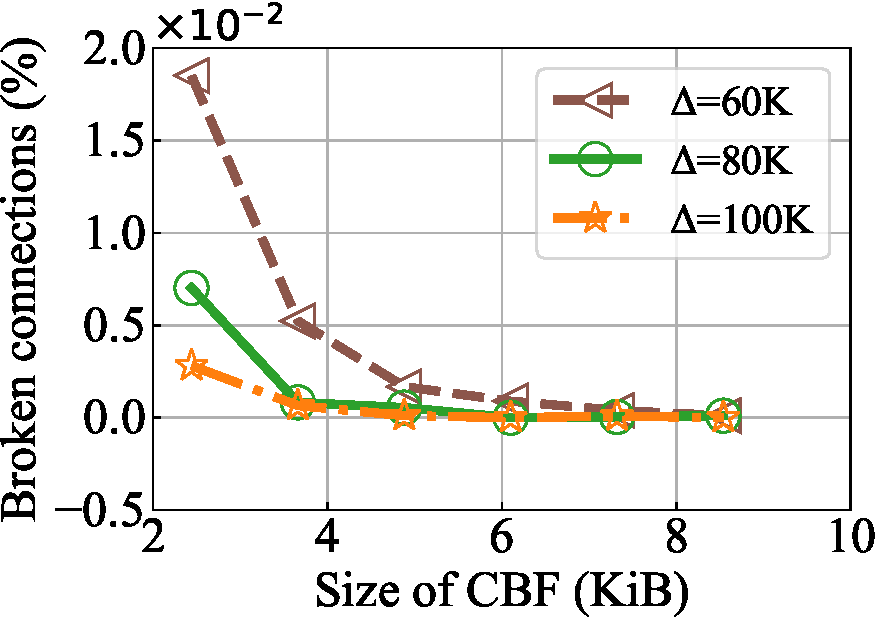
\includegraphics[width=1\linewidth]{experiment/5maatbrokenconn131072wb.pdf}
 		\end{minipage}
 		\label{10.1}
 	}
 	\subfigure[Data Mining.]{
 		\begin{minipage}{0.46\linewidth}
 			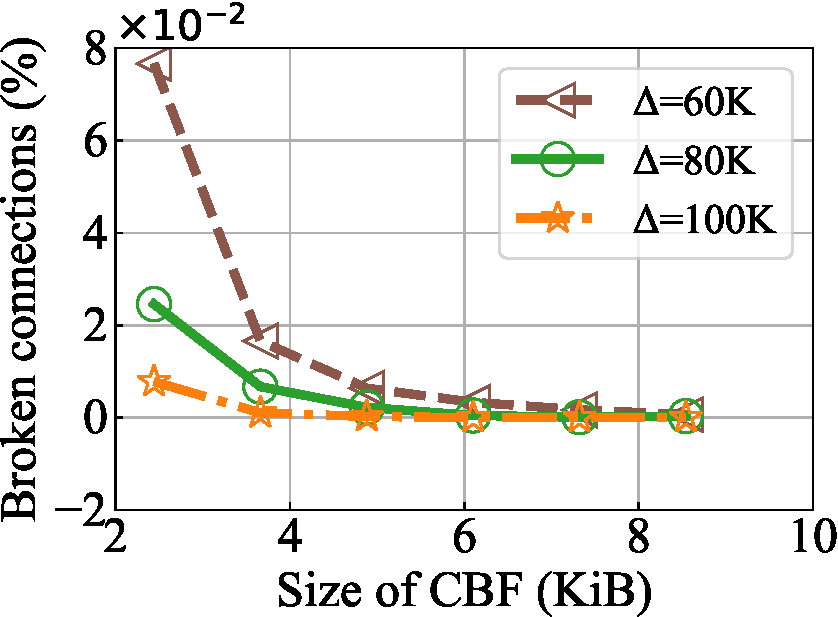
\includegraphics[width=0.98\linewidth]{experiment/5maatbrokenconn131072dm.pdf}
 		\end{minipage}
 		\label{10.2}
 	}
 	\caption{Broken connections ratio for the increasing size of CBF (2.44 KiB$\sim$8.54 KiB).}
 	\label{10}
 \end{figure}

\begin{figure}[t]
	\setlength{\abovecaptionskip}{0pt}
	\setlength{\belowcaptionskip}{-10pt}
	\centering
	\begin{minipage}{0.49\linewidth}
		\centering
		% height=1.8in, width=1.8in
		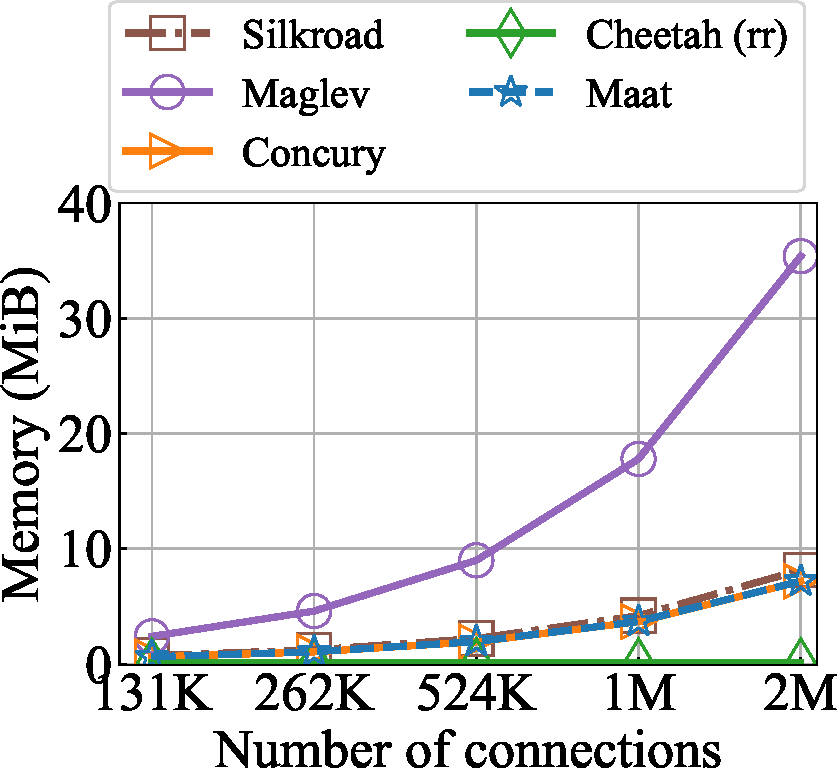
\includegraphics[width=1\linewidth]{experiment/6maatmemory.pdf}
		\caption{Memory cost of various schemes.}
		\label{11}%文中引用该图片代号
	\end{minipage}
	%\qquad
	\begin{minipage}{0.49\linewidth}
		\centering
		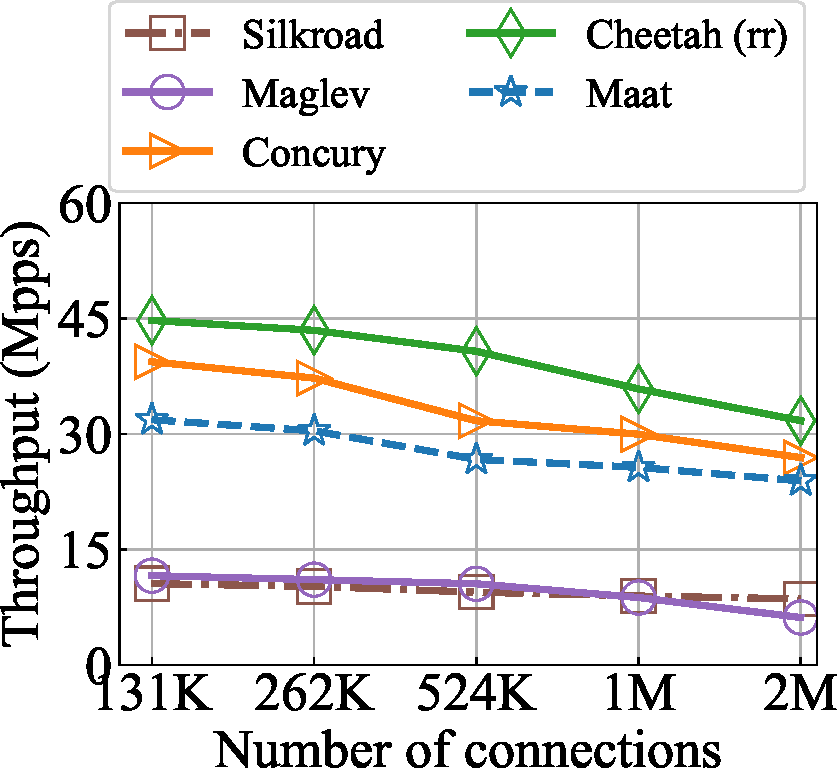
\includegraphics[width=1\linewidth]{experiment/7maatprocess.pdf}
		\caption{Process throughput of various schemes.}
		\label{12}%文中引用该图片代号
	\end{minipage}
\end{figure}

\textbf{PCC Violations under the different workload.} Avoiding PCC violations is a key feature of L4 LB. Maat does not experience broken connections when the DIP pool updates, but the power of one random choice brings potential broken connections. We solve this problem using CBF. Therefore, we evaluated the memory overhead required by CBF to fully guarantee PCC under heavy load (130K connections) before the next data plane update. The results are shown in Fig. \ref{10}. When $\Delta$ is 100K packets, CBF only needs 5.6 KiB memory overhead to fully guarantee PCC under both workloads. The main reason is that in Maat, only a small part of traffic (1.59\%) requires CBF insertion. For modern servers, a few KiB of memory overhead is negligible. Table II shows the PCC violations of several existing typical LB schemes \cite{barbette2021cheetah, shi2020concury}. Similar to Concury and Cheetah, Maat can guarantee 100\% PCC when sufficient memory resources are provided. However, Concury struggles to achieve better fairness, while Cheetah requires modifications to the existing protocol stack.

\begin{table}[htbp]
	\centering
	\caption{Broken connections ratio of various schemes.}
	\begin{tabular}{|c|c|} %l(left)居左显示 r(right)居右显示 c居中显示
		\hline 
		Schemes&Broken connections\\
		\hline  
		Hash (\cite{patel2013ananta, gandhi2015rubik})&11\%\\
		\hline
		Consistent-Hash (\cite{eisenbud2016maglev})&3\%\\
		\hline
		Concury (\cite{shi2020concury})&0\%\\
		\hline
		Cheetah (\cite{barbette2021cheetah})&0\%\\
		\hline
		Maat&0\%$\sim$0.0766\%\\
		\hline
	\end{tabular}
	\label{1}
	\vspace{0em}
\end{table}

\begin{figure*}[h]
	\setlength{\abovecaptionskip}{0pt}
	\setlength{\belowcaptionskip}{-10pt}
	%  for a heavy-tailed workload.
	\centering
	\begin{minipage}{0.245\textwidth}
		\centering
		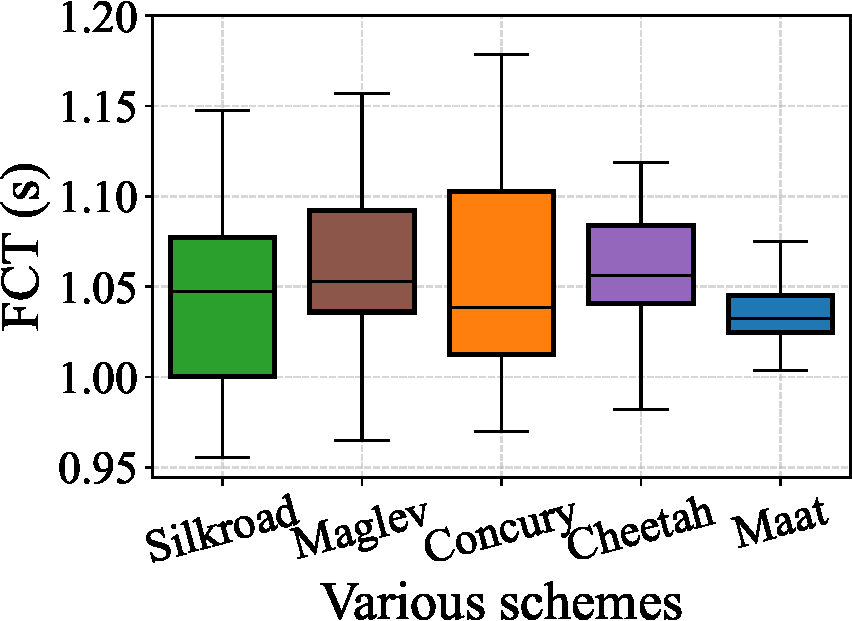
\includegraphics[width=1\textwidth]{experiment/8boxplotfct.pdf}
		\caption{Evaluation of various L4 LB schemes.}
		\label{13}
	\end{minipage}
	%\qquad
	\begin{minipage}{0.245\textwidth}
		\centering
		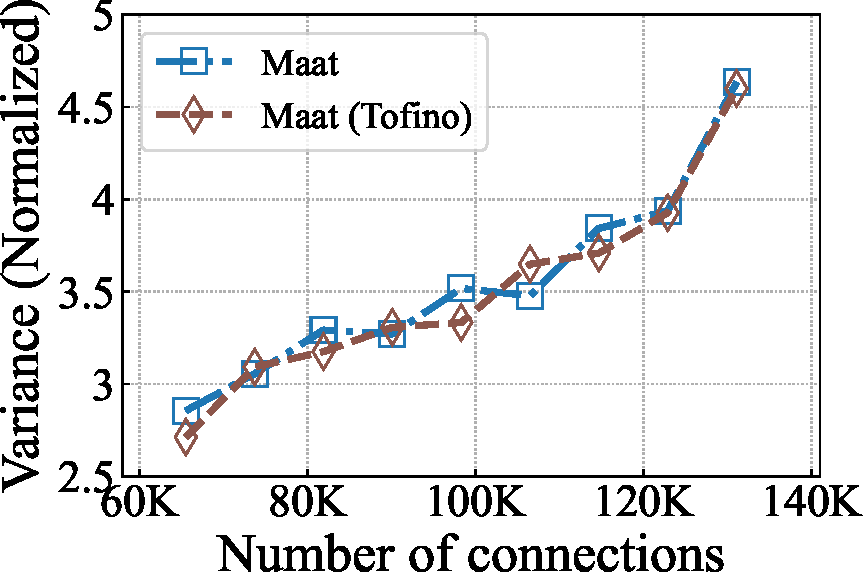
\includegraphics[width=1\textwidth]{experiment/9var.pdf}
		\caption{Variance of Maat and Maat (Tofino).}
		\label{14}
	\end{minipage}
	\begin{minipage}{0.245\textwidth}
		\centering
		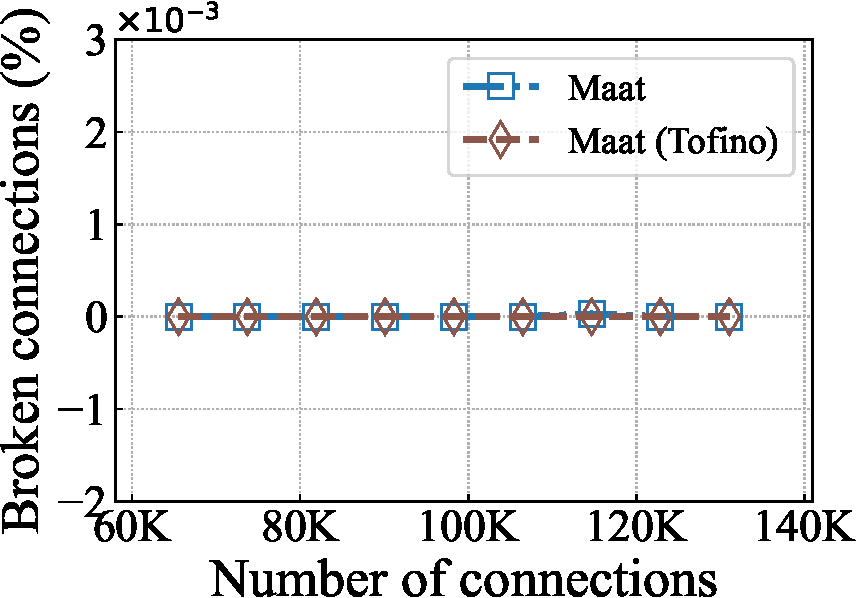
\includegraphics[width=1\textwidth]{experiment/10broken.pdf}
		\caption{Broken connections ratio of Maat and Maat (Tofino).}
		\label{15}
	\end{minipage}
	\begin{minipage}{0.245\textwidth}
		\centering
		% height=1.5in, width=1.8in
		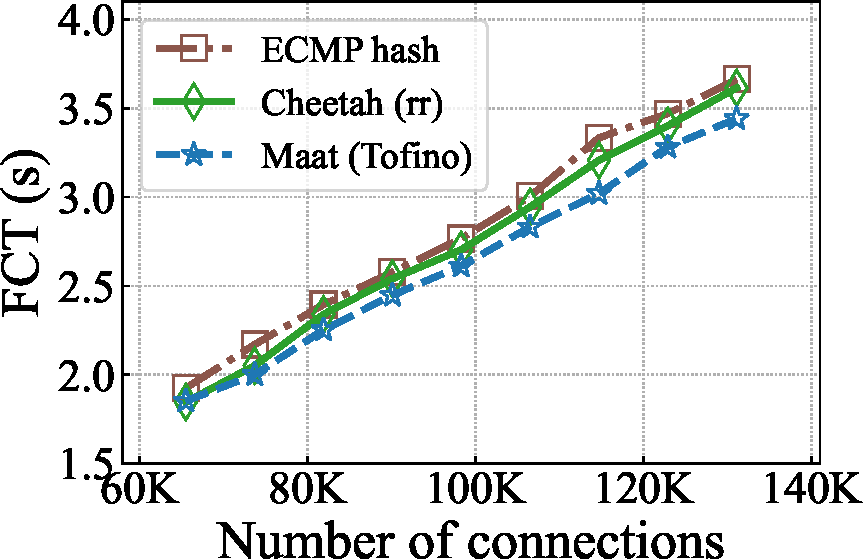
\includegraphics[width=1\textwidth]{experiment/11tofinofct.pdf}
		\caption{Flow completion time for Tofino experiment.}
		\label{16}
	\end{minipage}
\end{figure*}

\subsection{Evaluation of DPDK implementation}
Maat runs on a dual-socket Intel Xeon Silver 4210R CPU @ 2.40GHz, with a total of 40 logical CPU cores (10 cores per socket). We implement Maat using the Data Plane Development Kit (DPDK), a series of libraries for fast user-space packet processing \cite{pktgenDPDK}. In this testbed, we connect two commodity servers (\emph{S1} and \emph{S2}) to the Maat, and the configuration information is the same as the server where Maat is located. The Servers are connected via 100G Mellanox Connect-X 5 NICs. Logically, \emph{S1} acts as a client and \emph{S2} emulates 32 backend servers (DIPs). To evaluate the memory overhead and processing throughput of LB, we use Pktgen-DPDK \cite{pktgenDPDK} on the \emph{S1} to generate traffic and send them to the \emph{S2} through the LB. To evaluate flow completion time, we generated HTTP requests through WRK on \emph{S1}, and each core of \emph{S2} performs a constant amount of CPU-intensive work to schedule the 8KB file \cite{barbette2020high}.

\textbf{Memory Usage.} Fig. \ref{11} shows the memory cost required to store different connections for Maglev, SilkRoad, Concury, Cheetah, and Maat respectively. Cheetah does not need to maintain the mapping relationship between connections and servers as it stores the DIP in the packet header. Therefore, the memory resources occupied by Cheetah do not increase as the number of connections increases. To maintain PCC, the remaining schemes need to maintain the mapping relationship between connections and DIPs on LBs. As the number of connections increased, we found that the memory cost of Maglev is 79.75\% higher than the other three schemes. SilkRoad, Concury, and Maat occupy similar storage spaces. Compared with Concury, Maat introduces the following additional memory overhead: 1) State information about the DIPs needed to improve fairness; 2) CBF. When the number of connections is 1.04 million, the Maat additional overhead only accounts for 0.18\% of the total overhead. However, it can improve fairness by about 70\% compared to Concury.

\textbf{Process Throughput.} We also investigated the processing throughput of different L4 LB schemes. The higher the processing throughput, the fewer LBs we need to deploy. In this experiment, the metric is millions of packets per second (Mpps). In Fig. \ref{12}, we found that Cheetah (rr) has a 24.63\% improvement over Maat because it does not need to perform operations such as inserting and querying table entries in LB. However, it cannot be ignored that the actual deployment of Cheetah requires modification of the protocol stack. In contrast, Maat is easy to implement without any changes to end-hosts or protocol stack, and can be incrementally deployed in existing networks. Compared with Concury, the throughput of Maat is reduced by 14.01\% due to additional compute-intensive operations required to improve the fairness of server loads. However, compared with Maglev and Silkroad, Maat's operations on the data plane are simpler, resulting in improvements of 65.09\% and 60.5\%, respectively.

\textbf{Maat improves flow completion time with heavy-tailed workloads.} Fig. \ref{13} shows the distribution of flow completion times for 32 servers. \emph{S1} uses WRK to generate heavy-tail distributed HTTP requests (130K connections). For Maglev, Silkroad, and Concury, we find that some servers in these three schemes have high FCT, which verifies that hash-based LB has poor fairness performance as mentioned above, while the FCT of Maat is improved by up to 10.58\% compared to these solutions. Compared with these hash-based schemes, the improvement of Cheetah (rr) is not significant, because under heavy-tailed distribution, some servers are loaded unpredictably, and Cheetah (rr) struggles to cope with this scenario. This experiment demonstrates the advancement of the scheduling method (power of one random choice) used in Maat, which can help us make full use of the resources of all servers.

\begin{table}[tbp]
	\centering
	\caption{Resource consumption of Maat and Cheetah (rr).}
	\begin{tabular}{|c|c|c|} %l(left)居左显示 r(right)居右显示 c居中显示
		\hline 
		Resource&Maat&Cheetah (rr)\\
		\hline  
		Hash Bits&3.8\%&2.1\%\\
		\hline
		Gateway &8.3\%&4.2\%\\
		\hline
		SRAM &2.2\%&1.8\%\\
		\hline
		VLIW Actions&6.0\%&2.6\%\\
		\hline
		ALU Instruction&12.5\%&4.2\%\\
		\hline
	\end{tabular}
	\label{1}
	\vspace{-1em}
\end{table}

\subsection{Evaluation of Tofino implementation}
We implemented Maat on the Tofino target, where the data plane contains about 700 lines of P4 code. Due to the limitation of hardware resources that are exclusively accessed at all stages of the pipeline, we did not count the first packet of each flow, but this did not affect our measurement of the load on different servers. In Fig. \ref{14} and Fig. \ref{15}, we compare the hardware implementation (Maat (Tofino)) and the ideal implementation (Maat), and we can find that our compromised implementation on the Tofino switch does not affect the improvement of fairness and the maintenance of PCC. We use thrift to implement communication between the data plane and the control plane. Once a DIP pool update event occurs, the ASDP needs to be changed, which is done by the control plane through the thrift API. Maat also uses the thrift API to clear the CBF and update the DIP_table to forward new connections to the correct DIP. In this experiment, we use the WRK HTTP request generator on one machine as the client and 32 cores of another machine as the 32 servers, where the two servers are connected through a Tofino switch.

Maat is compared with the following two methods in this experiment: 1) a simple hash-based LB implemented in P4; 2) stateless Cheetah using round-robin (rr), with an increasing number of connections for 1MB files. Table III shows the hardware resource usage of the packet processing pipeline at the programmable switch under Maat and Cheetah (rr). Maat uses more matching action tables and stages in the pipeline to implement comparison and calculation logic. These operations require more stateful ALU and SRAM, resulting in higher consumption of resources such as gateway, SRAM, and ALU instructions. In short, compared to Cheetah (rr), Maat consumes more hardware resources due to fine-grained scheduling of incoming traffic. However, the limited resource consumption is acceptable compared to the benefits of load balancing. In Fig. \ref{16}, we observe that FCT of Maat has a 9.67\% improvement compared to hash-based LB and still a 6.01\% improvement compared to Cheetah with round-robin. Maat achieves better FCT under higher loads because it takes advantage of the opportunities brought by random selection to more fully utilize all available server resources.

\section{CONCLUSION}
This paper presents Maat, an efficient Layer-4 load balancer for data center networks. By proposing a new scheduling method called the power of one random choice, Maat does not compromise fairness to maintain PCC as hash-based load balancers do. Moreover, Maat does not need to modify the existing protocol stack to introduce more advanced schedule mechanisms. Maat also introduces CBF to distinguish which traffic is forwarded to hash-selected servers and which traffic is forwarded to randomly selected servers, resolving potential PCC violations. We implemented Maat on both a software prototype and a programmable ASIC Tofino switch. The evaluation results show that compared with other existing L4 LBs, Maat can fully maintain PCC at cost of negligible memory overhead and significantly improve fairness.


\bibliographystyle{ieeetr}
\bibliography{ref}



\end{document}
